
\documentclass{article} % For LaTeX2e
\usepackage{iclr2027_conference,times}

% Optional math commands from https://github.com/goodfeli/dlbook_notation.
\input{math_commands.tex}

\usepackage{hyperref}
\usepackage{url}
\usepackage{array}
\usepackage{graphicx}
\usepackage{longtable}
\hypersetup{hidelinks}


\title{Graph-Based KV Cache Compression\\with Answer Supervision}

% Authors must not appear in the submitted version. They should be hidden
% as long as the \iclrfinalcopy macro remains commented out below.
% Non-anonymous submissions will be rejected without review.

\author{Daniel Ohayon \\
Department of Computer Science\\
Ben-Gurion University of the Negev\\
Beer-Sheva, Israel \\
\texttt{danieloh@post.bgu.ac.il} \\
\AND
Daniel Boharon \\
Department of Computer Science\\
Ben-Gurion University of the Negev\\
Beer-Sheva, Israel \\
\texttt{bohadan@post.bgu.ac.il} \\
\AND
Moshe Eliasof \\
Department of Computer Science\\
Ben-Gurion University of the Negev\\
Beer-Sheva, Israel \\
\texttt{eliasof@bgu.ac.il} \\
}

% The \author macro works with any number of authors. There are two commands
% used to separate the names and addresses of multiple authors: \And and \AND.
%
% Using \And between authors leaves it to \LaTeX{} to determine where to break
% the lines. Using \AND forces a linebreak at that point. So, if \LaTeX{}
% puts 3 of 4 authors names on the first line, and the last on the second
% line, try using \AND instead of \And before the third author name.

\newcommand{\fix}{\marginpar{FIX}}
\newcommand{\new}{\marginpar{NEW}}

% \iclrfinalcopy % Uncomment for camera-ready version, but NOT for submission.
\begin{document}


\maketitle

\begin{abstract}
Language-model agents perform multistep tasks by accumulating conversation histories, retrieved documents, and tool outputs. As these contexts grow, the key–value (KV) cache becomes a substantial memory bottleneck. Compression is particularly challenging in these settings: information introduced early may support later decisions, and relevant evidence may be distributed across multiple observations. These demands motivate cache eviction policies that consider relationships among tokens and their utility for subsequent generation. We introduce a method that uses graph neural networks (GNNs) to guide KV cache compression. Building on FastKVzip, our selector augments token representations through message passing before predicting retention scores. Training proceeds in two stages. First, a warm-up stage uses importance scores computed by KVzip’s context reconstruction procedure as supervision, providing an informed starting point for cache selection. Second, answer-supervised fine-tuning aligns the selector with the underlying language model’s generation behavior: the selector learns to retain information that allows the model to reproduce answers generated with its full cache. The language model remains frozen throughout, while the selector is trained across varying compression budgets. Our approach thus connects relational reasoning over context with supervision from the model’s own answers, targeting the preservation of task-relevant information within a limited cache.
\end{abstract}

\section{Introduction}
\label{sec:introduction}

Language-model agents build solutions over a sequence of interactions: they retrieve evidence, invoke tools, inspect observations, and revise their next actions. Frameworks such as ReAct make this interaction between reasoning and environmental feedback explicit \citep{yao2023react}, while memory-management systems address the difficulty of maintaining useful information over extended sessions \citep{packer2023memgpt}. The accumulated history is therefore part of the agent's working context. Keeping this context available incurs a growing cost: autoregressive Transformers store key--value (KV) representations of previous tokens to avoid recomputing them during decoding, and this cache grows with the sequence length. Efficient cache management is consequently central to serving long interactions under a fixed memory budget \citep{kwon2023pagedattention}.

The compression problem is not determined by context length alone. A tool output may contain a fact needed several actions later, and an answer may depend on evidence spread across different observations. Recency and relevance to the current question can therefore provide incomplete guidance about what to retain. Query-agnostic compression addresses this setting by constructing a compressed cache before a particular downstream question is known \citep{kim2025kvzip}. The objective is to preserve information that the language model can use across subsequent requests, while removing cache entries whose contribution does not justify their memory cost.

KVzip estimates this contribution by asking the underlying language model to reconstruct the context and measuring how strongly cached entries are attended to during reconstruction \citep{kim2025kvzip}. Fast KVzip learns a lightweight gate to predict these scores from hidden representations, avoiding reconstruction when scoring a new context \citep{kim2026fastkvzip}. Its gate operates separately on each token representation. These representations already contain context from the frozen Transformer, but the selector itself does not learn an additional exchange of information across token positions. This motivates examining whether explicit relational modeling within the selector can better support cache retention decisions.

We develop a graph-based cache selector that augments Fast KVzip with learned message passing within context blocks. Tokens form the nodes of a graph whose edge weights depend on their hidden representations. Separate graph parameters for each layer and KV head allow the selector to represent different relationships within the same context. The resulting messages enrich the representations used to predict retention scores; the retained KV vectors themselves remain unchanged. Graph-based eviction has also been explored through similarity-based score propagation \citep{li2025graphkv}. Our focus is on learning the relational scoring function and adapting its decisions to the behavior of the frozen language model.

Training has two stages with distinct roles. Reconstruction-score supervision first serves as a warm-up, providing direct targets for individual cache entries and an informed starting point for the selector. Answer supervision then adapts this selector to downstream generation: given a context and question, the full-cache model supplies a reference answer, and the selector is trained so that the same model can predict that answer from a compressed cache. The question supplies training feedback without becoming an input to the context selector. This separates a broadly available importance signal from an objective tied to how the model uses the retained information.

\medskip
\noindent\textit{[Final introduction paragraph reserved for the principal empirical findings and the paper's main contributions.]}


\section{Related Work}
\label{sec:related}

\subsection{Attention Mechanism and KV Caching}
Consider a context of $T$ tokens and a Transformer layer $\ell$ with hidden states $X^{(\ell)}\in\mathbb{R}^{T\times d}$. In multi-head attention, head $h$ at this layer uses learned projections to form query, key, and value matrices~\citep{vaswani2017attention}:
\begin{equation}
    Q_h=X^{(\ell)}W_{Q,h},\qquad
    K_h=X^{(\ell)}W_{K,h},\qquad
    V_h=X^{(\ell)}W_{V,h}.
    \label{eq:qkv-projections}
\end{equation}
Each projection maps the hidden states to a head dimension $d_h$; normalization and positional transformations are omitted here for clarity.

During autoregressive decoding, the current token's query $q_{T,h}$, the $T$-th row of $Q_h$, computes the head output
\begin{equation}
    o_{T,h}=\operatorname{softmax}\!\left(
    \frac{q_{T,h}K_h^{\top}}{\sqrt{d_h}}
    \right)V_h,
    \label{eq:cached-attention}
\end{equation}
where $K_h$ and $V_h$ contain the keys and values up to position $T$, including the current token. Causal attention makes earlier representations depend only on their prefixes, so appending a token leaves their keys and values unchanged. These can therefore be reused from the KV cache, to which only the current key and value are appended. Earlier queries need not be retained: each decoding step uses its own query to read the stored keys and values. Grouped-query attention (GQA) further reduces cache storage by sharing key and value projections among groups of query heads~\citep{ainslie2023gqa}.

Attention heads can serve different functions~\citep{voita2019heads}. For example, DuoAttention identifies retrieval heads that need access to distant tokens and streaming heads that can rely on recent tokens and a few initial attention sinks~\citep{xiao2025duoattention}. A token's importance can therefore differ across heads, motivating retention decisions specific to each layer and KV head.

\subsection{Soft Token Compression}
Soft compression represents a long context through a shorter sequence of continuous representations. AutoCompressors learn summary vectors that condition subsequent language modeling~\citep{chevalier2023autocompressors}. The In-context Autoencoder (ICAE) maps context to compact memory slots using reconstruction and language-model pretraining followed by instruction fine-tuning~\citep{ge2024icae}. Latent Context Language Models (LCLMs) train encoder--decoder compressors at scale and use the resulting latent tokens as context for a decoder~\citep{li2026lclm}. RestoreKV complements retained KV entries with a small learned restore cache, trained against full-cache answer distributions while keeping the evictor fixed~\citep{baek2026restorekv}. These approaches synthesize representations that can combine information from multiple tokens. Our approach learns which original KV entries to retain. Message passing changes the selector's representations while preserving the retained keys and values.

\subsection{Hard Token Compression}
Compression can also operate on discrete text or internal model states. At the text level, summarization rewrites a history into a shorter description, whereas extractive prompt compression removes portions of the original input. LLMLingua performs budgeted, iterative token deletion before the target model processes the prompt~\citep{jiang2023llmlingua}. Pruning can instead occur within a model: FastV, for example, removes visual-token representations after early layers of a vision--language model~\citep{chen2024fastv}. Such approaches differ in what is removed and when the compression cost is incurred.

KV eviction directly removes stored key--value pairs. H$_2$O combines accumulated attention importance with recency~\citep{zhang2023h2o}; StreamingLLM retains initial attention sinks and a recent window for bounded-memory streaming~\citep{xiao2024streamingllm}; and SnapKV selects important positions using attention from a prompt-end observation window~\citep{li2024snapkv}. Maintaining fluent streaming generation and preserving evidence for arbitrary future questions are different objectives. KVzip explicitly addresses query-agnostic cache reuse by scoring KV entries through context reconstruction~\citep{kim2025kvzip}. Fast KVzip learns lightweight gates to predict these scores from hidden states~\citep{kim2026fastkvzip}, and KVzap also learns an efficient approximation to KVzip~\citep{jegou2026kvzap}. Learned eviction has additionally been optimized through generation objectives: DMS uses output-distribution supervision~\citep{lancucki2025dms}, while TRIM-KV trains retention gates with prediction and distribution-matching losses~\citep{bui2026trimkv}. Our method builds on Fast KVzip's scoring framework, adding relational token modeling and a reconstruction-supervised warm-up followed by supervision from full-cache reference answers.

\paragraph{Graph-based selection.}
Message-passing neural networks update node representations by aggregating information from their neighbors~\citep{gilmer2017mpnn}. Graph Isomorphism Networks (GINs) combine a node's own representation with summed neighborhood features before a learned transformation~\citep{xu2019gin}, motivating our aggregation-and-update design. Graph-based KV selection also has direct precedent: GraphKV~\citep{li2025graphkv} propagates similarity-based decay signals from selected tokens to discourage redundant retention. Our focus is a learned graph selector whose message-passing transformations and retention scores are optimized through reconstruction supervision and subsequent answer-supervised adaptation.


\section{Method}
\label{sec:method}

We consider a frozen autoregressive Transformer with $L$ layers and $H$ KV heads. Prefilling a context of $T$ tokens, $c=(c_1,\ldots,c_T)$, produces a cache $\mathcal{C}(c)$ and hidden representations $X^{\ell}\in\mathbb{R}^{T\times d}$. Compression is applied after this prefill, producing a cache for subsequent questions. A selector with parameters $\theta$ assigns a score $s_{\ell h i}$ to each context entry. Compression retains a subset of the original KV pairs according to these scores and a retention budget $\rho$. The selector observes the context before the downstream question is supplied. System-prefix entries and subsequently appended question and answer tokens lie outside the context budget.

\subsection{Fast KVzip Gating Mechanism}
\label{sec:gate}

Fast KVzip predicts KV importance from token representations using a low-dimensional sink-attention gate~\citep{kim2026fastkvzip}. Fix a layer $\ell$ and KV head $h$, and write $x=x_i^{\ell}$. Suppressing these indices on the projection parameters, the gate forms a key and $G$ queries, where $G$ is the number of query heads sharing the KV head:
\begin{equation}
    \widehat{\mathbf q}_j=\operatorname{RMSNorm}_{\ell}^{q}\!\left(xW_j^q+\mathbf b_j^q\right),\qquad
    \widehat{\mathbf k}=\operatorname{RMSNorm}_{\ell}^{k}\!\left(xW^k\right),
    \label{eq:gate-features}
\end{equation}
with $W_j^q,W^k\in\mathbb{R}^{d\times d_g}$ and gate width $d_g$. RMSNorm rescales each projected vector by its root-mean-square magnitude and applies learned featurewise scales. These are auxiliary gate features.

Let $\boldsymbol\kappa_1,\ldots,\boldsymbol\kappa_S\in\mathbb{R}^{d_g}$ be learned reference keys, shared across token positions. With the token-key logit $a_j=\langle\widehat{\mathbf q}_j,\widehat{\mathbf k}\rangle/\sqrt{d_g}+b_j$ and learned scalar bias $b_j$, the gate used here is
\begin{equation}
    s_{\ell h i}=g_{\ell h}(x_i^{\ell})=
    \frac{1}{G}\sum_{j=1}^{G}
    \frac{\exp(a_j)}{\exp(a_j)+\sum_{m=1}^{S}
    \exp\!\left(\langle\widehat{\mathbf q}_j,\boldsymbol\kappa_m\rangle/\sqrt{d_g}\right)}.
    \label{eq:fastkvzip-gate}
\end{equation}
Each fraction measures the attention mass assigned to the token's key in competition with the reference keys; averaging yields one importance score per KV head. The frozen Transformer supplies contextual representations, which this gate scores separately at each position. Our graph module enriches these representations through message passing before applying the same mapping $g_{\ell h}$.

\subsection{Graph-Based Token Mixing}
\label{sec:mixing}

\subsubsection{Graph Construction}

We partition the context into contiguous blocks $\mathcal{B}$ and apply the same selector parameters to each block. A single block can also cover the entire context. For one block $b\in\mathcal{B}$ of $T_b=|b|$ tokens, suppress the layer and head indices and write its representations as $X\in\mathbb{R}^{T_b\times d}$. Learned projections $W_a,W_v\in\mathbb{R}^{d\times r}$ produce relation features $U$ and message features $R$:
\begin{equation}
    U=XW_a,\qquad R=XW_v,\qquad A=\frac{1}{T_b}UU^{\top}.
    \label{eq:graph}
\end{equation}
Here $A_{ij}$ is the weight of the connection between tokens $i$ and $j$. The relation projection is learned across contexts, while the graph is recomputed from the representations of each input. Every layer--KV-head pair has its own projections. The adjacency is symmetric, can contain signed weights, and includes self-connections. These weights define learned feature interactions rather than probabilities or prescribed semantic relations.

\subsubsection{Message Passing and Retention Scores}

With $W_o\in\mathbb{R}^{r\times d}$, we aggregate messages and form a residual update:
\begin{equation}
    P=ARW_o,\qquad
    X'=X+\alpha\,\operatorname{LeakyReLU}\!\left(\operatorname{BatchNorm}(P)\right),\qquad
    s_{\ell h i}=g_{\ell h}(x'_i).
    \label{eq:mixer}
\end{equation}
BatchNorm~\citep{ioffe2015batchnorm} uses the current block's token statistics during both training and inference. The scalar $\alpha$, normalization parameters, and message projections are specific to each layer--KV-head pair. This update follows the aggregation-and-update structure of message-passing networks \citep{gilmer2017mpnn,xu2019gin}; the learned weighted graph specifies which token features contribute to each message. We evaluate message passing in factorized form without constructing the adjacency matrix, giving a cost linear in block length for fixed feature dimensions (Appendix~\ref{app:factorized}).

The residual changes only the auxiliary representations used for scoring. The language model's hidden states and retained KV vectors are not replaced by mixed features. Scores from all blocks are concatenated before eviction, so graph blocks do not impose separate retention quotas. Given a retention ratio $\rho$, a uniform per-head budget retains the $k=\max(1,\lfloor\rho T\rfloor)$ highest-scoring context entries in each layer and KV head. The scores also support a shared budget across layers and heads, allowing nonuniform retention. Selected entries keep their original order and positional information. Block boundaries restrict the selector's message passing, while its input representations retain the contextual information supplied by the frozen Transformer.

\begin{figure}[t]
    \centering
    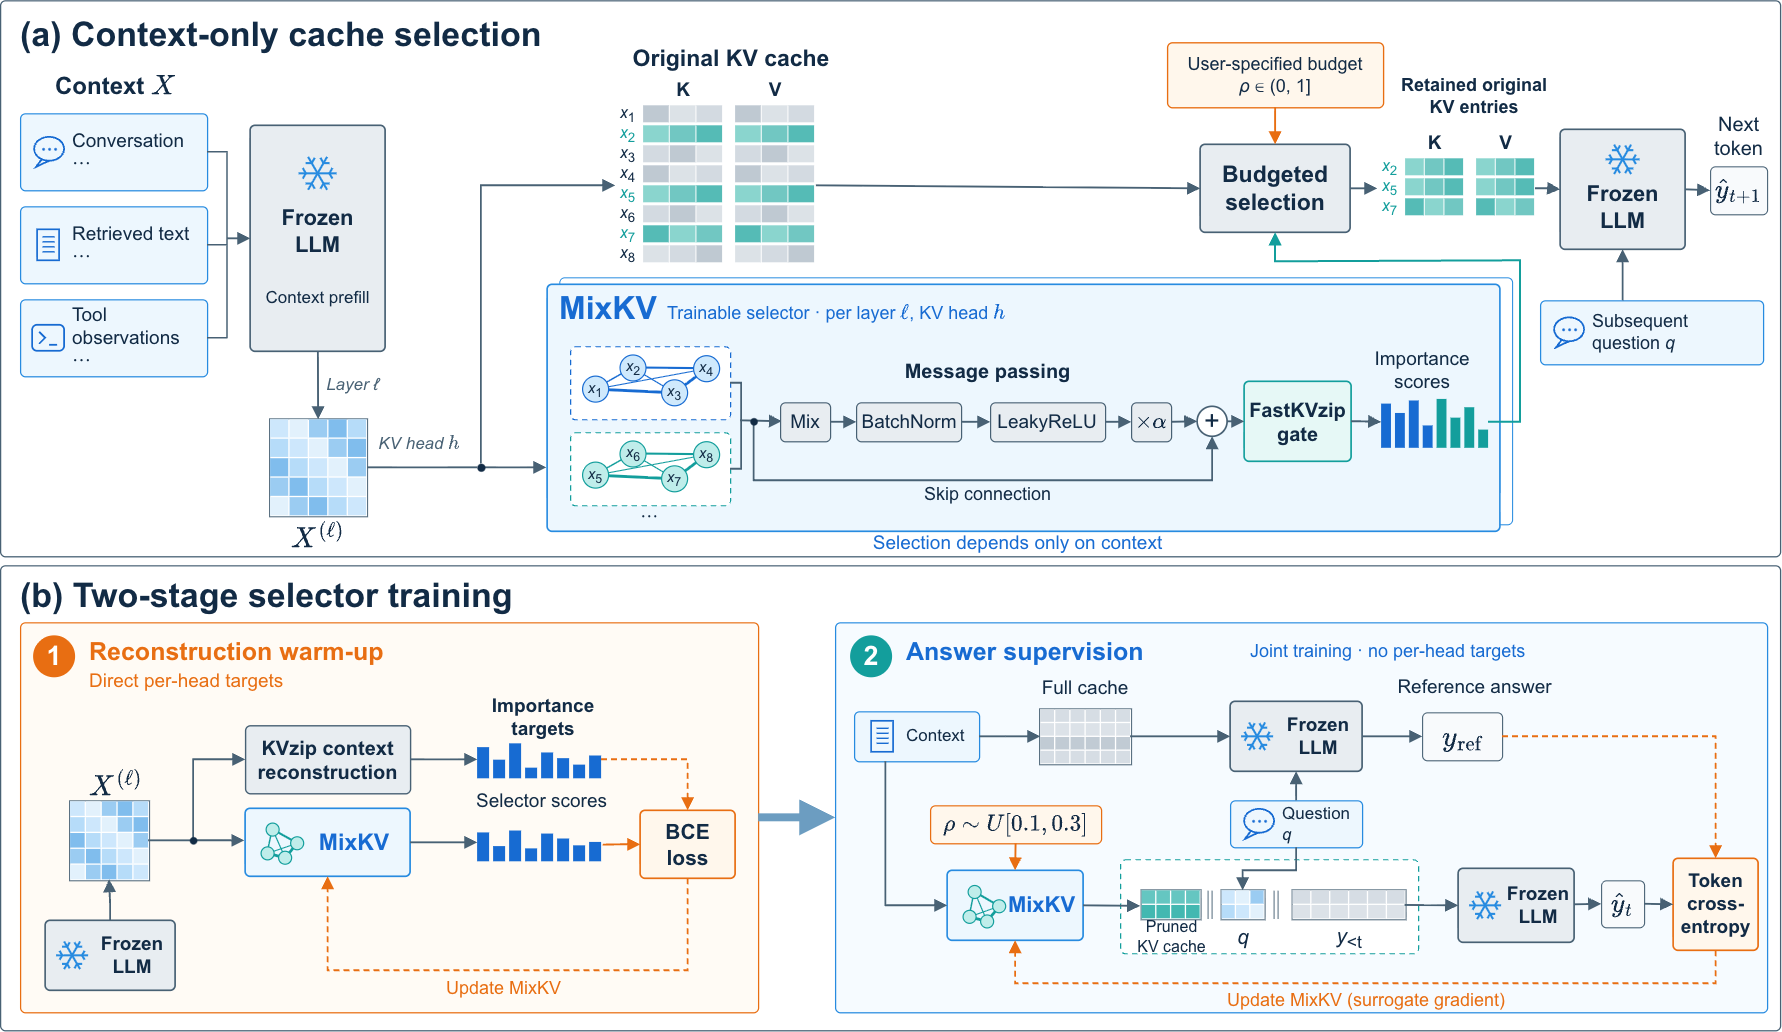
\includegraphics[width=\linewidth]{figures/mixkv-overview.png}
    \caption{\textbf{MixKV architecture and training.}
    (a) A trainable selector mixes context-token representations through message passing and scores them with a Fast KVzip gate. Budgeted selection retains original KV entries before a subsequent question is supplied.
    (b) Reconstruction-score supervision warms up the selector, followed by answer supervision from the frozen full-cache model using a straight-through surrogate. The language model remains frozen in both stages.}
    \label{fig:overview}
\end{figure}

\subsection{Two-Stage Training}
\label{sec:training}

\subsubsection{Stage 1: Reconstruction-Supervised Warm-Up}

KVzip computes an importance target $t_{\ell h i}\in[0,1]$ from the maximum attention received by a cached entry during context reconstruction, aggregating over reconstruction positions and the query heads that share that KV head \citep{kim2025kvzip}. Following Fast KVzip, we use these scores as continuous targets for binary cross-entropy. For a collection of training blocks, the objective is
\begin{equation}
    \mathcal{L}_{\mathrm{warm}}=
    -\frac{1}{|\mathcal{B}|LH}\sum_{b\in\mathcal{B}}\sum_{\ell,h}
    \frac{1}{T_b}\sum_{i\in b}
    \left[t_{\ell h i}\log s_{\ell h i}+(1-t_{\ell h i})\log(1-s_{\ell h i})\right].
    \label{eq:warmup}
\end{equation}
Both the graph mixer and gate are trained, with the gate optionally initialized from Fast KVzip. Reconstruction supervision supplies a direct target for each cache entry and gives the selector an informed starting point. These targets express the reconstruction procedure's assessment of importance; reproducing them alone does not directly optimize answers generated from a compressed cache.

\subsubsection{Stage 2: Answer Supervision}

For a context--question pair $(c,q)$, the frozen language model with its full cache generates a reference answer $y^*$. We then compress the context cache using the selector and train on the reference answer under teacher forcing:
\begin{equation}
    \mathcal{L}_{\mathrm{ans}}(\theta)=
    -\frac{1}{|y^*|}\sum_{t=1}^{|y^*|}
    \log p_{\phi}\!\left(y_t^*\mid q,y_{<t}^*,\mathcal{C}_{\theta}(c;\rho)\right),
    \label{eq:answerloss}
\end{equation}
where $\phi$ denotes the frozen language-model parameters. Only answer tokens contribute prediction loss. The question and reference prefix condition the prediction, and gradients update the mixer and gate. We vary $\rho$ across training examples, either by sampling a retention interval or by following a decreasing schedule. This stage aligns cache selection with the model's ability to predict its full-cache answers, rather than requiring continued agreement with reconstruction scores. It uses reference sequences, not a loss matching the teacher's complete output distribution. Answer supervision is query-dependent during training, but the learned selector remains a function of the context alone.

To train through hard top-$k$ selection, we use a straight-through surrogate that preserves the retained KV entries in the forward pass while supplying score gradients during backpropagation (Appendix~\ref{app:surrogate}). We then recompute the selector one graph block at a time and replay these score gradients, limiting live selector activations to one block (Appendix~\ref{app:replay}).


\section{Experimental Results}

\subsection{Setup}

Datasets, models, baselines (including a summary baseline where the model is asked to summarize the context and then answers the question based on the summary - watch out for varying retention ratio of the summary)

The reported suite combines RULER \citep{hsieh2024ruler}, SCBench
\citep{li2025scbench}, and LongBench v2 \citep{bai2024longbenchv2}.
Appendix~\ref{app:benchmarks} explains every supported
task and length variant, summarizes context lengths, and identifies the
configurations still missing from the
matched three-method comparison. All 27 prepared SCBench configurations
are reported, spanning mean context lengths from approximately 7K to 169K
Qwen tokens.

\subsection{Main Results}
\label{sec:main-results}

Tables~\ref{tab:results-graphkv}--\ref{tab:results-kvzip} in
Appendix~\ref{app:benchmark-results} report all 60 evaluated configurations
separately for our graph-based selector, Fast KVzip, and KVzip. Each table
includes the complete per-task curves, benchmark-level macro-averages, and
the method's own uncompressed baseline; no scores are averaged across
retention ratios. Appendix~\ref{app:retention-curves} provides the corresponding
retention--score curves, benchmark summaries, and official task-family groupings.

All three methods use Qwen2.5-7B-Instruct-1M and the same prepared benchmark
splits: all 13 RULER tasks at both 4K and 8K, seven selected tasks at 64K,
and all 27 prepared SCBench configurations (11 base tasks and 16 length
variants). Every RULER configuration contains 500
examples. The complete suite contains 18,531 contexts and 28,236 questions
per method. The comparison preserves each deployed method's evaluation
procedure: our selector and KVzip prune after full-context prefill, while
Fast KVzip uses its native chunked-prefill eviction with 16,000-token
chunks. Our selector and Fast KVzip use a protected local window of 2\%;
KVzip uses no protected window. Thus this is a comparison of method
pipelines, not an ablation that isolates the scoring architecture.

For the 11 SCBench base tasks, we additionally evaluate 5\% and 10\%
retention, extending Tables~\ref{tab:results-graphkv}--\ref{tab:results-kvzip}
with two columns and Appendix~\ref{app:retention-curves} with two points on
the corresponding 11 base-task panels, their aggregate mean, and their four
family panels. This extension covers these 11 configurations only: the 16
SCBench length variants and all 33 RULER configurations were not evaluated
at these two ratios, and the corresponding table cells and curves are
unaffected. As with the rest of the comparison, no scores are averaged
across retention ratios.

Scores are on a 0--100 scale. Aggregate rows are unweighted means of the
included configuration scores at each retention ratio. SCBench is summarized
both over its 11 base tasks and over all 27 configurations; the latter gives
equal weight to each length variant. These and the selected RULER aggregate
are descriptive prepared-split summaries, not official complete-benchmark
scores. Mixed SCBench tasks retain one configuration score each, and
Summary + needles retains the inherited 48-token output cap for both summary
and retrieval questions. Full-cache scores are
reported separately for each method rather than assumed to be identical.

\paragraph{Context-length comparison.}
Figure~\ref{fig:context-score-buckets} pools individual context examples
from all 60 configurations into buckets of their measured token lengths.
To account for differences in task difficulty, we divide each method's
mean score within each configuration and bucket by its own full-cache mean
on the same contexts. We then average these relative scores with weights
proportional to the number of contexts per configuration in the bucket.
Thus 100\% denotes full-cache performance; values above 100\% are retained.
Scores use the native evaluator, including the equal-component mean for
RepoQA + KV, and retention ratios are plotted separately. This preserves
equal context weighting after normalization and differs from the
configuration-level macro-averages in the tables. Task composition and
sample counts still vary by bucket, so these curves describe the mixed
suite rather than isolating the effect of context length.

On the seven RULER tasks shared by our 4K, 8K, and 64K evaluations
(single~1, multikey~3, multivalue, VT, CWE, FWE, and QA~2), the score gap
to KVzip at 20\% retention changes from $-3.41$ and $-3.46$ points to
$+2.81$ points, respectively. This suggests stronger relative performance
at longer contexts, but not a universal scaling trend: gains over Fast
KVzip are mixed, and task composition and retention ratio matter.

\paragraph{LongBench v2.}
The benchmarks above are dominated by retrieval. LongBench v2
\citep{bai2024longbenchv2} instead asks 503 four-way multiple-choice questions
that require understanding and reasoning over realistic long contexts:
single- and multi-document QA, long in-context learning, long dialogue
history, code repositories, and structured data, with contexts from 8K to
2M words. We evaluate all 503 questions with the same checkpoint, protected
windows, and chunking as above, truncate contexts to the model's 1M-token
limit (the longest raw context has 4.2M tokens), ask for the answer
directly without chain-of-thought, and decode greedily for up to 128
tokens. The score is accuracy on a 0--100 scale, so one question is
0.2 points. The unpruned model reaches 30.22 (152/503), only
5.2 points above the 25-point chance level, which leaves little
room for pruning to hurt. Every pruned configuration in
Table~\ref{tab:longbench-v2} lies within 2.8 points of the full cache,
the largest gap between methods at any ratio is 2.6 points, and no
method leads at every ratio (GraphKV at 20\%, 30\%, and 75\%; KVzip at 40\% and 50\%). The clearest separation is at
20\% retention, where GraphKV is 0.2 points below the full cache
while Fast KVzip loses 1.0 and KVzip 2.8 points; across the
five ratios GraphKV's scores span 1.6 points, Fast KVzip's 1.8,
and KVzip's 4.4. These differences amount to a handful of questions,
and we do not read a ranking from them. What this benchmark shows is that
aggressive pruning leaves long-context multiple-choice accuracy essentially
unchanged for all three selectors.

\begin{table}[t]
\caption{LongBench v2 accuracy (0--100) on all 503 questions at each retention ratio; the last column is the unpruned model. One question is 0.2 points.}
\label{tab:longbench-v2}
\centering
\small
\begin{tabular}{@{}lrrrrrr@{}}
\hline
Method & 20\% & 30\% & 40\% & 50\% & 75\% & Full \\
\hline
GraphKV (ours) & 30.02 & 30.42 & 30.42 & 29.82 & 31.41 & 30.22 \\
Official FastKVzip & 29.22 & 30.02 & 30.42 & 31.01 & 31.01 & 30.22 \\
KVzip & 27.44 & 29.62 & 30.82 & 31.81 & 30.82 & 30.22 \\
\hline
\end{tabular}
\end{table}


\subsection{Efficiency}

Show time taken from prefill start to the point we have pruned KV cache (just before generation). Compare to other methods like KVzip, FastKVzip, and summarizing the context.

\subsection{Summarization Alignment To The Underlying LLM}
\label{sec:summarization-alignment}

The benchmarks in Section~\ref{sec:main-results} are dominated by retrieval: a fact is planted in a
long context and the model is asked to recover it. Such tasks establish that a pruned cache retains
specific tokens, but they say little about whether the model still represents the context as a
whole. We therefore evaluate a task with no single answer span. Each model is asked to summarise a
long document in roughly 400--500 words, and we ask how far pruning moves the summary away from what
the unpruned model would have written.

\paragraph{Setup.} We summarise 493 GovReport documents and 77 PG-19 books, each at least $8{,}192$
tokens long, under all three selectors and five retention ratios, plus the full cache. Decoding uses
temperature $0.7$, top-$p$ $0.9$ and up to $1{,}024$ new tokens, and we draw $N = 16$ samples per
document per condition, giving $164{,}160$ summaries over $1{,}710$ method--document records. All
three methods see exactly the same documents, so every comparison below is paired.

\paragraph{The unpruned model is not a fixed reference.} At temperature $0.7$ the full cache does not
agree with itself: two independent full-cache summaries of the same GovReport document share a
ROUGE-L F1 of only $0.318$. A raw full-versus-pruned score of $0.300$ at $20\%$ retention
therefore looks catastrophic while being almost exactly what resampling alone produces. We
consequently report every metric normalised by the full cache's agreement with itself. For one
document, let $B$ be the mean score over the $\binom{16}{2} = 120$ full-cache pairs with distinct
sample indices and $C$ the mean over all $16 \times 16 = 256$ full-versus-pruned pairs at a given
ratio; we report $100\,C/B$, averaged over documents with equal weight. A value of $100$ means
pruning perturbs the summary no more than resampling the unpruned model does, and values slightly
above $100$ are admissible.

\paragraph{Metrics.} We measure content with BERTScore F1 (\texttt{roberta-large}, layer 17, no IDF
weighting and no baseline rescaling), local phrasing with ROUGE-2 F1, wording and word order with
complete-summary ROUGE-L F1, and writing style with the cosine similarity of StyleDistance
embeddings. Summaries run a median of roughly $700$ tokens against a $512$-token encoder window, so
both neural metrics are computed over non-overlapping $510$-token windows covering every token
rather than by truncating; for a summary that fits a single window this reduces exactly to the
published metric, which we verify to $2.9\times10^{-8}$ against the reference implementation.

\paragraph{Pruning changes wording, not content.} Table~\ref{tab:summarization-alignment} shows that
all three selectors stay at or above $99$ on every metric down to $30\%$ retention, on both
datasets. The interesting behaviour is at $20\%$, and only on GovReport, where the metrics separate:
GraphKV loses $5.1$ points of ROUGE-2 and $5.5$ points of ROUGE-L, but only
$0.4$ points of BERTScore, while style does not move at all. The summaries are being
reworded rather than emptied of content. An evaluation restricted to $n$-gram overlap would have
reported this as a five-point degradation.

\paragraph{Two metrics saturate.} This normalisation is only informative where the baseline leaves
room. Full-cache self-agreement is $0.898$ for BERTScore and $0.987$ for StyleDistance, and no
StyleDistance cell departs from $100$ by more than $0.1$. The flat style result is an absence of
measurement range rather than evidence that style is preserved, and we report it for completeness
only.

\paragraph{Method differences do not support a ranking.} Because the cohort is paired over 493
documents, the comparison is sensitive enough to resolve differences of roughly $0.05$ normalised
points, and $35$ of the $120$ method comparisons in the grid are individually significant
after a Bonferroni correction. Their signs, however, are not stable: on GovReport BERTScore, GraphKV
leads FastKVzip by $+0.038$ at $75\%$ retention, trails it by $-0.142$ at $30\%$, and leads again by
$+0.069$ at $20\%$, with every one of those differences clearing the corrected threshold. Across all
significant lexical and BERTScore comparisons GraphKV is ahead in 14 and behind in 8. We therefore
do not read an overall ordering out of this experiment. The one setting in which an ordering is
consistent is the most aggressive ratio: at $20\%$ retention on GovReport, GraphKV leads both
baselines on all three informative metrics simultaneously
(Table~\ref{tab:summarization-significance}).

\paragraph{Scope.} Every metric here measures similarity to the unpruned model's own output. None
measures factual accuracy, faithfulness to the source document, or summary quality, and none would
detect an error that the unpruned model also makes. These results bound how far pruning moves the
model from itself; they do not establish that the resulting summaries are good.

\begin{table}[t]
\caption{Summarization alignment to the full-cache model. Each cell is $100\,C/B$: the mean similarity between full-cache and pruned-cache summaries of the same document ($C$, 256 sample pairs), divided by the full-cache pool's agreement with itself ($B$, 120 pairs), computed per document and then averaged with equal document weight. $100$ means pruning perturbs the output no more than resampling the unpruned model does. Column $B$ reports the raw full-cache self-agreement, the scale on which each metric operates.}
\label{tab:summarization-alignment}
\centering
\small
\begin{tabular}{@{}llrrrrrr@{}}
\hline
Metric & Method & $B$ & 20\% & 30\% & 40\% & 50\% & 75\% \\
\hline
\multicolumn{8}{@{}l}{\emph{GovReport (493 documents per method)}} \\
BERTScore F1 & GraphKV (ours) & 0.898 & 99.63 & 99.74 & 99.90 & 99.96 & 100.01 \\
 & Official FastKVzip & 0.898 & 99.56 & 99.89 & 99.96 & 99.96 & 99.97 \\
 & KVzip & 0.898 & 99.50 & 99.84 & 99.95 & 100.01 & 100.00 \\
\noalign{\smallskip}
ROUGE-2 F1 & GraphKV (ours) & 0.307 & 94.88 & 98.42 & 99.97 & 99.93 & 100.07 \\
 & Official FastKVzip & 0.306 & 93.81 & 98.76 & 99.59 & 99.32 & 99.48 \\
 & KVzip & 0.307 & 93.56 & 98.37 & 99.49 & 99.60 & 99.84 \\
\noalign{\smallskip}
ROUGE-L F1 & GraphKV (ours) & 0.318 & 94.52 & 97.37 & 99.03 & 99.32 & 100.14 \\
 & Official FastKVzip & 0.318 & 93.46 & 97.96 & 99.02 & 98.91 & 99.46 \\
 & KVzip & 0.318 & 93.05 & 97.50 & 98.73 & 99.22 & 99.95 \\
\noalign{\smallskip}
StyleDistance cosine & GraphKV (ours) & 0.987 & 100.02 & 99.91 & 99.94 & 99.99 & 100.02 \\
 & Official FastKVzip & 0.987 & 100.04 & 100.01 & 99.98 & 99.99 & 100.00 \\
 & KVzip & 0.987 & 100.04 & 99.99 & 99.99 & 100.03 & 100.01 \\
\hline
\multicolumn{8}{@{}l}{\emph{PG-19 (77 documents per method)}} \\
BERTScore F1 & GraphKV (ours) & 0.885 & 99.74 & 99.83 & 99.93 & 99.97 & 99.99 \\
 & Official FastKVzip & 0.885 & 99.66 & 99.90 & 100.01 & 99.99 & 99.96 \\
 & KVzip & 0.885 & 99.79 & 99.93 & 99.97 & 99.97 & 100.00 \\
\noalign{\smallskip}
ROUGE-2 F1 & GraphKV (ours) & 0.226 & 97.74 & 99.33 & 99.99 & 100.15 & 100.07 \\
 & Official FastKVzip & 0.226 & 96.19 & 99.23 & 100.23 & 100.06 & 99.30 \\
 & KVzip & 0.226 & 98.31 & 100.52 & 100.67 & 100.37 & 99.93 \\
\noalign{\smallskip}
ROUGE-L F1 & GraphKV (ours) & 0.264 & 98.24 & 99.14 & 99.40 & 99.86 & 100.08 \\
 & Official FastKVzip & 0.264 & 97.73 & 99.52 & 100.00 & 99.84 & 99.59 \\
 & KVzip & 0.264 & 98.36 & 99.42 & 99.84 & 100.02 & 100.04 \\
\noalign{\smallskip}
StyleDistance cosine & GraphKV (ours) & 0.988 & 100.02 & 100.01 & 100.04 & 100.06 & 100.02 \\
 & Official FastKVzip & 0.988 & 100.03 & 100.03 & 100.04 & 100.02 & 100.00 \\
 & KVzip & 0.988 & 100.05 & 100.04 & 100.01 & 100.00 & 100.03 \\
\hline
\end{tabular}
\end{table}

\begin{table}[t]
\caption{Paired method differences at $20\%$ retention on GovReport, the one setting where an ordering is consistent across metrics. Differences are paired over the 493 documents scored under every method; intervals are $95\%$ bootstrap confidence intervals over documents ($10{,}000$ resamples). All six clear a Bonferroni-corrected threshold of $p < 4.17\times10^{-4}$ for the 120 comparisons in the grid.}
\label{tab:summarization-significance}
\centering
\small
\begin{tabular}{@{}llr@{\,}l@{}}
\hline
Metric & GraphKV & \multicolumn{2}{c}{Difference (95\% CI)} \\
\hline
BERTScore F1 & vs.\ Official FastKVzip & $+0.069$ & $[+0.048, +0.091]$ \\
 & vs.\ KVzip & $+0.123$ & $[+0.092, +0.151]$ \\
ROUGE-2 F1 & vs.\ Official FastKVzip & $+1.072$ & $[+0.777, +1.368]$ \\
 & vs.\ KVzip & $+1.316$ & $[+0.890, +1.710]$ \\
ROUGE-L F1 & vs.\ Official FastKVzip & $+1.056$ & $[+0.788, +1.329]$ \\
 & vs.\ KVzip & $+1.468$ & $[+1.103, +1.823]$ \\
\hline
\end{tabular}
\end{table}


\subsection{Decoding Intensive Tasks}

Take benchmarks when the model needs to reason in many tokens and do the compaction every X tokens. This is modeling a scenario of an agent running in a long session.

\subsection{What Graph Structure is Being Learned}

Find a mathematical metric to report, or some figures that can tell something about what relations are being learned in every head and how similar the structures are across different grouped-query heads, heads, and different layers.

\subsection{Ablations}

\subsubsection{Effect of 2-stage training}

Train only stage 1, show results.

Train only stage 2, show results.

\subsubsection{Effect of GNN}

Train only stage 1 our model, show results compared to FastKVzip.

Take the 2 checkpoints (ours and FastKVzip) and train stage 2 on top of the pretrained checkpoint. See what contributes more - the architecture or the training methodology.

\newpage

\subsection*{AI use statement}

(This section is \textbf{required} and does not count toward the page limit.)

In this work, we used generative AI tools for [tasks with required disclosure].
We have not used generative AI tools for [other tasks with required disclosure],
and [the rest of the required disclosure tasks] are not applicable to this work.
Additionally, we used generative AI tools for [tasks with recommended
disclosure]. We have reviewed all AI-assisted work. [Elaborate. For example, “we
checked LLM-generated research ideas for potential plagiarism through a manual
literature survey”, “LLM-generated code was verified and tested for correctness
by 2 authors”, etc.]. We take responsibility for the final content of this work,
including text, claims or artifacts produced with the aid of generative AI.

See the ICLR 2027 AI Policy for Authors for more details. This statement should
not be more than 1 page.

\subsection*{Ethics statement}

(This section is \textbf{recommended} and does not count toward the page limit.)

If authors feel that their paper submission raises questions regarding the Code
of Ethics, they are encouraged to include a paragraph of Ethics Statement (at
the end of the main text before references) to address potential concerns where
appropriate. Topics include, but are not limited to, studies that involve human
subjects, practices to data set releases, potentially harmful insights,
methodologies and applications, potential conflicts of interest and sponsorship,
discrimination/bias/fairness concerns, privacy and security issues, legal
compliance, and research integrity issues (e.g., IRB, documentation, research
ethics). This statement should not be more than 1 page.

\subsection*{Reproducibility statement}

(This section is \textbf{recommended} and does not count toward the page limit.)

It is important that the work published in ICLR is reproducible. Authors are
strongly encouraged to include a paragraph-long Reproducibility Statement at the
end of the main text (before references) to discuss the efforts that have been
made to ensure reproducibility. This paragraph should not itself describe
details needed for reproducing the results, but rather reference the parts of
the main paper, appendix, and supplemental materials that will help with
reproducibility. For example, for novel models or algorithms, a link to an
anonymous downloadable source code can be submitted as supplementary materials;
for theoretical results, clear explanations of any assumptions and a complete
proof of the claims can be included in the appendix; for any datasets used in
the experiments, a complete description of the data processing steps can be
provided in the supplementary materials. Each of the above are examples of
things that can be referenced in the reproducibility statement.

\subsubsection*{Author Contributions}
If you'd like to, you may include  a section for author contributions as is done
in many journals. This is optional and at the discretion of the authors.

\subsubsection*{Acknowledgments}
Use unnumbered third level headings for the acknowledgments. All
acknowledgments, including those to funding agencies, go at the end of the paper.


\bibliography{iclr2027_conference}
\bibliographystyle{iclr2027_conference}

\clearpage
\appendix
\section{Additional Method Details}
\label{app:method}

\subsection{BatchNorm and Graph Scope}
\label{app:normalization}

For a block $b$ with $T_b=|b|$ tokens, the BatchNorm operator in Equation~\ref{eq:mixer} computes a population mean and variance separately for each output feature $j$:
\begin{equation}
    \mu_j=\frac{1}{T_b}\sum_{i=1}^{T_b}P_{ij},\qquad
    \sigma_j^2=\frac{1}{T_b}\sum_{i=1}^{T_b}(P_{ij}-\mu_j)^2,\qquad
    \operatorname{BatchNorm}(P)_{ij}=\gamma_j\frac{P_{ij}-\mu_j}{\sqrt{\sigma_j^2+\epsilon}}+\beta_j.
\end{equation}
We use $\epsilon=10^{-5}$ for numerical stability. Means and variances are recomputed on the current block at inference; there are no running statistics. The featurewise affine parameters $\gamma,\beta$ and scalar residual coefficient $\alpha$ are learned for each layer--KV-head pair. Normalization and its affine transform precede LeakyReLU. The original representation is added outside the activation.

The graph adjacency $UU^{\top}/T_b$ is positive semidefinite, but its individual edge weights can be negative. Its diagonal is retained. Our update is a weighted message-passing operator with a learned residual; it is not the standard GIN architecture, and GIN's expressivity results do not establish an equivalent guarantee for this selector \citep{xu2019gin}. Independent graph blocks restrict which positions exchange new messages. This architectural choice is distinct from dividing the computation of a fixed graph into smaller token batches, which preserves that graph's normalization domain.

\subsection{Learning Through Discrete Cache Selection}
\label{app:surrogate}

Hard top-$k$ selection does not provide a useful ordinary derivative with respect to the scores. We use a straight-through surrogate \citep{bengio2013straightthrough} that leaves the compacted cache unchanged in the forward pass. Suppressing layer and head indices, define scaled softmax weights
\begin{equation}
    a_i=k\frac{\exp(s_i/\tau)}{\sum_{j=1}^{T}\exp(s_j/\tau)},\qquad
    \widetilde{K}_i=K_i,\qquad
    \widetilde{V}_i=\left[1+a_i-\operatorname{sg}(a_i)\right]V_i,
    \quad\text{for retained }i,
    \label{eq:ste}
\end{equation}
where $\operatorname{sg}$ is the identity in the forward pass with zero derivative, and $\tau>0$ controls the surrogate's smoothness. The multiplier is exactly one during prediction, and only selected entries are present. During backpropagation, the value multipliers provide a gradient to the scores. The shared softmax denominator also gives unselected scores an indirect competitive signal. The selected keys and discrete indices have no score-gradient path. This is a biased surrogate for learning a discrete selection policy; it is not an exact derivative of top-$k$.

\paragraph{Score gradient of the surrogate.}
Let $\mathcal{I}$ denote the retained indices for one layer and KV head, and let $\pi_i=\operatorname{softmax}(s/\tau)_i$, so that $a_i=k\pi_i$ in Equation~\ref{eq:ste}. The weights $a_i$ sum to $k$ and can exceed one; they are not Bernoulli retention probabilities. For a selected entry, define
\begin{equation}
    c_i=\left\langle\frac{\partial\mathcal{L}_{\mathrm{ans}}}{\partial\widetilde{V}_i},V_i\right\rangle,
    \qquad i\in\mathcal{I}.
\end{equation}
Set $c_j=0$ for unselected entries. Since $\partial a_i/\partial s_j=(a_i/\tau)(\mathbf{1}_{i=j}-\pi_j)$, the surrogate score gradient is
\begin{equation}
    \frac{\partial\mathcal{L}_{\mathrm{ans}}}{\partial s_j}
    =\frac{1}{\tau}\left[
    \mathbf{1}_{j\in\mathcal{I}}c_j a_j
    -\pi_j\sum_{i\in\mathcal{I}}c_i a_i\right].
    \label{eq:scoregradient}
\end{equation}
The first term measures sensitivity through a retained value. The second couples all scores through softmax normalization, including scores of evicted entries. An evicted score can therefore receive feedback even though its value is absent from the forward cache. This feedback is indirect: it does not evaluate what the language model would have generated had that evicted entry been retained. The temperature changes this backward surrogate, not the temperature used to generate reference answers.

\subsection{Efficiency and Gradient Replay}
\label{app:efficiency}

\subsubsection{Factorized Message Passing}
\label{app:factorized}

The graph in Equation~\ref{eq:graph} need not be materialized. Associativity gives
\begin{equation}
    P=U\left(\frac{U^{\top}R}{T_b}W_o\right).
    \label{eq:factorized}
\end{equation}
The intermediate contraction is $r\times r$, avoiding storage of a $T_b\times T_b$ adjacency. For one layer--head pair, projection and message computation require $O(T_bdr+T_br^2+r^2d)$ operations, linear in block length for fixed feature widths. Tokenwise scoring adds another linear pass. This bound concerns the selector's message computation; it does not include cache selection or imply linear-time Transformer prefill.

\paragraph{Forward workspace.}
For forward scoring without retained activation graphs, one active layer--head pair can retain $U$ with $O(T_br)$ entries, the $r\times r$ contraction, and the $r\times d$ output kernel. Normalization statistics require $O(d)$ storage. Streaming the remaining feature-width operations in batches of $m$ tokens requires $O(md)$ additional workspace, rather than storing every intermediate of size $T_b\times d$. With blocks of maximum size $B$, the message computation across a context costs
\begin{equation}
    O\!\left(LH\left[Tdr+Tr^2+\left\lceil T/B\right\rceil r^2d\right]\right).
\end{equation}
This expression excludes the gate, cache selection, and frozen-model computation. The graph mixer has $3dr+2d+1$ learned parameters per layer--KV-head pair, independently of context length.

\subsubsection{Replaying Selector Gradients}
\label{app:replay}

Although the language model is frozen, answer supervision still requires differentiating its predictions with respect to the compressed cache. Keeping the selector's activation graph alive during that backward pass adds avoidable memory pressure. Write the concatenated score function as $s=\operatorname{concat}_{b\in\mathcal{B}}f_{\theta}(X_b)$, where $f_{\theta}$ is the block scorer. We first compute all selector scores without retaining their activation graph, then differentiate the answer loss with respect to a detached score tensor to obtain $u=\partial\mathcal{L}_{\mathrm{ans}}/\partial s$. After the language-model backward pass, we recompute the selector one independent block at a time and apply the saved score gradients:
\begin{equation}
    \nabla_{\theta}\mathcal{L}_{\mathrm{ans}}
    =\sum_{b\in\mathcal{B}}
    J_{f_{\theta}(X_b)}^{\top}u_b.
    \label{eq:replay}
\end{equation}
Here $J$ is the block scorer's Jacobian with respect to $\theta$; it is applied without being explicitly formed. The answer loss can couple scores from all blocks through selection and the surrogate, but this cross-block competition is already represented in $u$. Once the full score derivative is available, the chain rule separates the remaining parameter gradient by independent scorer blocks. Each block is recomputed with the same parameters and normalization statistics as in the first pass, and only its corresponding slice $u_b$ is applied. Gradients accumulate across all blocks before the parameters are updated. With unchanged parameters and deterministic replay, this is an exact chain-rule rearrangement of the chosen surrogate gradient. Arbitrarily slicing a graph that contains cross-block edges would not satisfy this independence argument.

Replay trades an additional selector forward pass for retaining at most one block's scorer activation graph, following the recomputation principle of activation checkpointing \citep{chen2016checkpointing}. It does not repeat context prefill or the language-model backward pass for each block.

\paragraph{Full-context memory.}
Replay still requires $O(LHT)$ scalar scores and score gradients, the frozen hidden representations, and the original and compacted caches, all of which scale with context length, in addition to language-model answer activations and optimizer state. Consequently, this technique does not make total training memory independent of context length. A full-context graph can use the same replay separation, but its single block spans all $T$ tokens.

\paragraph{Streaming reconstruction-supervised gradients.}
The warm-up objective also permits recomputation within a fixed graph, provided normalization derivatives account for all its tokens. With $Z=(P-\mu)/\sqrt{\sigma^2+\epsilon}$ and $D=\partial\mathcal{L}_{\mathrm{warm}}/\partial Z$, the featurewise backward map is
\begin{equation}
    \frac{\partial\mathcal{L}_{\mathrm{warm}}}{\partial P}
    =\frac{1}{\sqrt{\sigma^2+\epsilon}}
    \left[D-\operatorname{mean}_{i}(D)-Z\odot\operatorname{mean}_{i}(D\odot Z)\right].
\end{equation}
The reductions are over the complete graph, even when projection and gate computations are replayed in smaller batches. This preserves the objective's normalization domain. Storage used by these gradient buffers is additional to the forward workspace above; a bound on factorized forward intermediates is not a bound on all training memory.

\clearpage
\section{Detailed Benchmark Results}
\label{app:benchmark-results}

Each table contains all 60 evaluated configurations. Bold aggregate rows are arithmetic means of unrounded configuration scores, computed independently for each column. SCBench 11-base-task mean excludes the 16 length variants; SCBench 27-configuration mean includes them equally. RULER selected 33 weights the 4K, 8K, and selected 64K groups by 13/33, 13/33, and 7/33. These are descriptive prepared-split summaries, not official complete-benchmark scores; the overall mean also mixes heterogeneous metrics. Display values are rounded only after aggregation.
The 5\% and 10\% columns are additionally reported for the 11 SCBench base-task configurations and their aggregate mean only. The 16 SCBench length variants and all 33 RULER configurations were not evaluated at these two ratios and show --- in both columns, as do the aggregate rows that include them.
Full-cache scores are method-specific.

\begingroup
\small
\setlength{\tabcolsep}{4pt}
\begin{longtable}{@{}lrrrrrrrr@{}}
\caption{Our graph-based selector: post-prefill pruning; 2\% protected local window. Absolute scores (0--100) for the complete selected suite.}
\label{tab:results-graphkv} \\
\hline
Benchmark / configuration & 5\% & 10\% & 20\% & 30\% & 40\% & 50\% & 75\% & Full (100\%) \\
\hline
\endfirsthead
\multicolumn{9}{l}{\tablename\ \thetable{} (continued)} \\
\hline
Benchmark / configuration & 5\% & 10\% & 20\% & 30\% & 40\% & 50\% & 75\% & Full (100\%) \\
\hline
\endhead
\hline
\multicolumn{9}{r}{\emph{Continued on next page}} \\
\endfoot
\hline
\endlastfoot
SCBench KV & 1.20 & 32.40 & 71.60 & 69.60 & 72.00 & 72.40 & 68.60 & 68.20 \\
SCBench KV (mid) & --- & --- & 63.20 & 68.60 & 70.40 & 70.60 & 69.20 & 68.90 \\
SCBench KV (short) & --- & --- & 70.50 & 83.40 & 85.30 & 86.30 & 84.70 & 85.50 \\
SCBench KV (tiny) & --- & --- & 68.20 & 85.90 & 89.70 & 90.20 & 88.90 & 88.00 \\
SCBench MF & 16.50 & 29.67 & 35.33 & 37.33 & 35.83 & 33.50 & 33.67 & 33.00 \\
SCBench MF (mid) & --- & --- & 35.50 & 36.83 & 35.00 & 32.67 & 34.33 & 34.83 \\
SCBench MF (short) & --- & --- & 38.67 & 37.83 & 36.50 & 34.67 & 37.00 & 37.83 \\
SCBench MF (tiny) & --- & --- & 40.00 & 40.50 & 39.00 & 37.33 & 38.33 & 39.50 \\
SCBench QA (English) & 12.23 & 27.29 & 42.51 & 45.64 & 42.85 & 45.00 & 44.02 & 42.92 \\
SCBench RepoQA & 2.05 & 38.86 & 55.68 & 58.64 & 59.55 & 59.55 & 59.77 & 59.09 \\
SCBench RepoQA (short) & --- & --- & 70.00 & 70.00 & 70.91 & 70.91 & 72.73 & 72.73 \\
SCBench RepoQA (tiny) & --- & --- & 64.44 & 73.33 & 75.56 & 71.11 & 75.56 & 75.56 \\
SCBench Summary & 27.65 & 32.22 & 36.05 & 36.30 & 36.23 & 36.51 & 36.77 & 36.82 \\
SCBench Summary (mid) & --- & --- & 40.36 & 40.60 & 39.76 & 39.94 & 39.95 & 39.17 \\
SCBench Summary (short) & --- & --- & 40.33 & 40.52 & 39.06 & 40.51 & 40.63 & 39.31 \\
SCBench Summary (tiny) & --- & --- & 38.08 & 38.21 & 36.95 & 38.29 & 38.34 & 37.12 \\
SCBench Choice (English) & 49.54 & 68.98 & 72.22 & 73.61 & 80.56 & 80.56 & 76.39 & 79.17 \\
SCBench Many-shot & 32.96 & 30.37 & 34.07 & 34.44 & 37.04 & 38.15 & 38.15 & 38.52 \\
SCBench Many-shot (short) & --- & --- & 32.96 & 33.70 & 35.56 & 36.67 & 34.81 & 35.56 \\
SCBench Many-shot (tiny) & --- & --- & 33.70 & 34.81 & 36.30 & 34.81 & 35.56 & 35.19 \\
SCBench Prefix/suffix & 0.60 & 10.80 & 30.00 & 42.80 & 43.40 & 40.00 & 44.80 & 51.20 \\
SCBench Prefix/suffix (mid) & --- & --- & 42.20 & 58.00 & 65.60 & 65.80 & 70.20 & 69.60 \\
SCBench Prefix/suffix (short) & --- & --- & 34.40 & 61.40 & 76.80 & 81.60 & 86.60 & 88.80 \\
SCBench Prefix/suffix (tiny) & --- & --- & 62.40 & 82.40 & 87.80 & 88.80 & 90.60 & 91.40 \\
SCBench VT & 40.00 & 45.96 & 42.31 & 40.44 & 41.07 & 41.78 & 41.38 & 41.29 \\
SCBench Summary + needles & 19.33 & 56.59 & 65.47 & 67.63 & 67.97 & 67.92 & 68.18 & 68.35 \\
SCBench RepoQA + KV & 3.55 & 52.41 & 74.86 & 79.26 & 80.11 & 80.40 & 81.25 & 80.82 \\
\hline
\textbf{SCBench 11-base-task mean} & \textbf{18.69} & \textbf{38.69} & \textbf{50.92} & \textbf{53.25} & \textbf{54.24} & \textbf{54.16} & \textbf{53.91} & \textbf{54.49} \\
\hline
\hline
\textbf{SCBench 27-configuration mean} & \textbf{---} & \textbf{---} & \textbf{49.45} & \textbf{54.51} & \textbf{56.18} & \textbf{56.15} & \textbf{56.68} & \textbf{56.98} \\
\hline
\pagebreak[4]
RULER 4K NIAH single 1 & --- & --- & 100.00 & 100.00 & 100.00 & 100.00 & 100.00 & 100.00 \\
RULER 4K NIAH single 2 & --- & --- & 100.00 & 100.00 & 100.00 & 100.00 & 100.00 & 100.00 \\
RULER 4K NIAH single 3 & --- & --- & 99.40 & 99.60 & 99.80 & 99.80 & 99.60 & 98.80 \\
RULER 4K NIAH multikey 1 & --- & --- & 96.00 & 98.40 & 98.60 & 99.20 & 99.20 & 99.00 \\
RULER 4K NIAH multikey 2 & --- & --- & 98.20 & 99.40 & 99.40 & 99.60 & 99.80 & 99.80 \\
RULER 4K NIAH multikey 3 & --- & --- & 98.00 & 98.80 & 98.80 & 99.40 & 99.60 & 99.60 \\
RULER 4K NIAH multivalue & --- & --- & 66.30 & 73.70 & 82.70 & 90.75 & 93.90 & 92.20 \\
RULER 4K NIAH multiquery & --- & --- & 99.50 & 99.70 & 99.95 & 99.90 & 99.90 & 100.00 \\
RULER 4K VT & --- & --- & 94.24 & 95.12 & 96.68 & 96.96 & 98.64 & 98.88 \\
RULER 4K CWE & --- & --- & 93.32 & 97.08 & 97.46 & 97.90 & 98.34 & 98.62 \\
RULER 4K FWE & --- & --- & 80.33 & 83.13 & 81.73 & 81.67 & 84.67 & 85.80 \\
RULER 4K QA 1 & --- & --- & 80.40 & 83.40 & 86.20 & 85.60 & 85.20 & 85.20 \\
RULER 4K QA 2 & --- & --- & 60.40 & 60.80 & 61.80 & 59.60 & 58.80 & 59.60 \\
\hline
\textbf{RULER 4K 13-task mean} & \textbf{---} & \textbf{---} & \textbf{89.70} & \textbf{91.47} & \textbf{92.55} & \textbf{93.11} & \textbf{93.67} & \textbf{93.65} \\
\hline
RULER 8K NIAH single 1 & --- & --- & 100.00 & 100.00 & 100.00 & 100.00 & 100.00 & 100.00 \\
RULER 8K NIAH single 2 & --- & --- & 100.00 & 100.00 & 100.00 & 100.00 & 100.00 & 100.00 \\
RULER 8K NIAH single 3 & --- & --- & 99.60 & 99.40 & 99.60 & 99.60 & 99.60 & 99.40 \\
RULER 8K NIAH multikey 1 & --- & --- & 96.00 & 98.20 & 98.80 & 98.80 & 99.40 & 99.60 \\
RULER 8K NIAH multikey 2 & --- & --- & 97.20 & 98.60 & 98.80 & 99.00 & 99.80 & 99.80 \\
RULER 8K NIAH multikey 3 & --- & --- & 90.80 & 95.40 & 95.80 & 95.80 & 97.00 & 97.20 \\
RULER 8K NIAH multivalue & --- & --- & 61.90 & 74.65 & 78.75 & 86.50 & 85.90 & 84.70 \\
RULER 8K NIAH multiquery & --- & --- & 99.60 & 99.75 & 99.85 & 99.95 & 99.95 & 99.90 \\
RULER 8K VT & --- & --- & 89.24 & 88.96 & 94.24 & 94.92 & 97.36 & 97.88 \\
RULER 8K CWE & --- & --- & 86.80 & 91.26 & 90.58 & 90.70 & 90.70 & 91.02 \\
RULER 8K FWE & --- & --- & 73.27 & 81.73 & 82.47 & 81.73 & 82.67 & 83.20 \\
RULER 8K QA 1 & --- & --- & 75.40 & 79.20 & 79.80 & 80.40 & 81.40 & 81.40 \\
RULER 8K QA 2 & --- & --- & 56.40 & 58.20 & 57.60 & 56.00 & 55.20 & 55.00 \\
\hline
\textbf{RULER 8K 13-task mean} & \textbf{---} & \textbf{---} & \textbf{86.63} & \textbf{89.64} & \textbf{90.48} & \textbf{91.03} & \textbf{91.46} & \textbf{91.47} \\
\hline
RULER 64K NIAH single 1 & --- & --- & 100.00 & 100.00 & 100.00 & 100.00 & 100.00 & 100.00 \\
RULER 64K NIAH multikey 3 & --- & --- & 89.00 & 90.40 & 92.40 & 91.80 & 91.80 & 91.60 \\
RULER 64K NIAH multivalue & --- & --- & 64.05 & 76.85 & 80.60 & 86.75 & 85.35 & 82.20 \\
RULER 64K VT & --- & --- & 80.28 & 78.80 & 79.32 & 80.28 & 78.32 & 77.04 \\
RULER 64K CWE & --- & --- & 36.74 & 42.80 & 42.08 & 38.50 & 27.74 & 33.80 \\
RULER 64K FWE & --- & --- & 80.93 & 85.53 & 86.47 & 87.07 & 86.53 & 86.00 \\
RULER 64K QA 2 & --- & --- & 47.60 & 49.20 & 48.00 & 48.60 & 47.60 & 46.60 \\
\hline
\textbf{RULER 64K selected 7 mean} & \textbf{---} & \textbf{---} & \textbf{71.23} & \textbf{74.80} & \textbf{75.55} & \textbf{76.14} & \textbf{73.91} & \textbf{73.89} \\
\hline
\hline
\textbf{RULER selected 33 mean} & \textbf{---} & \textbf{---} & \textbf{84.57} & \textbf{87.21} & \textbf{88.13} & \textbf{88.69} & \textbf{88.61} & \textbf{88.60} \\
\hline
\hline
\textbf{Overall selected 60 mean} & \textbf{---} & \textbf{---} & \textbf{68.77} & \textbf{72.50} & \textbf{73.75} & \textbf{74.05} & \textbf{74.24} & \textbf{74.37} \\
\hline
\end{longtable}
\endgroup
\clearpage

\begingroup
\small
\setlength{\tabcolsep}{4pt}
\begin{longtable}{@{}lrrrrrrrr@{}}
\caption{Fast KVzip: native chunked-prefill eviction; 2\% protected local window. Absolute scores (0--100) for the complete selected suite.}
\label{tab:results-fastkvzip} \\
\hline
Benchmark / configuration & 5\% & 10\% & 20\% & 30\% & 40\% & 50\% & 75\% & Full (100\%) \\
\hline
\endfirsthead
\multicolumn{9}{l}{\tablename\ \thetable{} (continued)} \\
\hline
Benchmark / configuration & 5\% & 10\% & 20\% & 30\% & 40\% & 50\% & 75\% & Full (100\%) \\
\hline
\endhead
\hline
\multicolumn{9}{r}{\emph{Continued on next page}} \\
\endfoot
\hline
\endlastfoot
SCBench KV & 2.80 & 32.80 & 47.00 & 66.80 & 66.40 & 72.80 & 68.20 & 68.20 \\
SCBench KV (mid) & --- & --- & 61.80 & 70.10 & 72.50 & 71.00 & 68.90 & 68.90 \\
SCBench KV (short) & --- & --- & 71.10 & 83.10 & 85.40 & 85.70 & 85.70 & 85.20 \\
SCBench KV (tiny) & --- & --- & 65.90 & 83.20 & 90.10 & 90.50 & 89.40 & 88.10 \\
SCBench MF & 19.33 & 29.33 & 32.83 & 33.50 & 34.00 & 33.83 & 32.83 & 33.00 \\
SCBench MF (mid) & --- & --- & 34.33 & 33.00 & 34.50 & 35.17 & 34.17 & 34.83 \\
SCBench MF (short) & --- & --- & 38.17 & 35.33 & 34.50 & 33.83 & 35.83 & 37.83 \\
SCBench MF (tiny) & --- & --- & 41.33 & 39.33 & 37.00 & 38.00 & 37.83 & 39.83 \\
SCBench QA (English) & 13.07 & 21.50 & 44.20 & 44.74 & 42.02 & 41.76 & 42.54 & 41.52 \\
SCBench RepoQA & 4.32 & 44.09 & 57.73 & 59.32 & 60.23 & 61.36 & 58.18 & 59.09 \\
SCBench RepoQA (short) & --- & --- & 69.09 & 67.27 & 70.00 & 71.82 & 72.73 & 72.73 \\
SCBench RepoQA (tiny) & --- & --- & 71.11 & 73.33 & 75.56 & 75.56 & 75.56 & 75.56 \\
SCBench Summary & 27.64 & 33.18 & 35.97 & 36.82 & 36.49 & 36.80 & 36.83 & 36.82 \\
SCBench Summary (mid) & --- & --- & 40.60 & 39.88 & 40.03 & 39.55 & 38.76 & 39.17 \\
SCBench Summary (short) & --- & --- & 40.60 & 39.88 & 40.03 & 39.55 & 38.76 & 39.17 \\
SCBench Summary (tiny) & --- & --- & 38.45 & 38.19 & 37.04 & 37.21 & 37.12 & 37.12 \\
SCBench Choice (English) & 46.30 & 68.98 & 73.61 & 75.00 & 75.00 & 75.00 & 79.17 & 79.17 \\
SCBench Many-shot & 34.81 & 32.59 & 33.70 & 36.67 & 37.04 & 36.30 & 36.30 & 38.52 \\
SCBench Many-shot (short) & --- & --- & 34.44 & 35.93 & 34.81 & 34.07 & 34.07 & 35.56 \\
SCBench Many-shot (tiny) & --- & --- & 34.07 & 34.44 & 32.96 & 33.70 & 35.19 & 35.19 \\
SCBench Prefix/suffix & 0.60 & 11.20 & 38.80 & 48.40 & 55.60 & 47.40 & 36.80 & 51.20 \\
SCBench Prefix/suffix (mid) & --- & --- & 47.80 & 63.20 & 74.80 & 70.80 & 67.20 & 69.60 \\
SCBench Prefix/suffix (short) & --- & --- & 45.00 & 62.00 & 80.20 & 85.00 & 88.00 & 88.80 \\
SCBench Prefix/suffix (tiny) & --- & --- & 64.00 & 80.40 & 88.80 & 90.00 & 92.00 & 91.40 \\
SCBench VT & 43.02 & 49.02 & 43.51 & 41.73 & 40.58 & 40.53 & 41.38 & 41.29 \\
SCBench Summary + needles & 16.96 & 54.54 & 65.64 & 68.29 & 67.86 & 67.56 & 68.17 & 68.35 \\
SCBench RepoQA + KV & 7.67 & 54.55 & 77.84 & 79.55 & 80.40 & 80.26 & 80.68 & 80.82 \\
\hline
\textbf{SCBench 11-base-task mean} & \textbf{19.68} & \textbf{39.25} & \textbf{50.08} & \textbf{53.71} & \textbf{54.15} & \textbf{53.96} & \textbf{52.83} & \textbf{54.36} \\
\hline
\hline
\textbf{SCBench 27-configuration mean} & \textbf{---} & \textbf{---} & \textbf{49.95} & \textbf{54.42} & \textbf{56.44} & \textbf{56.48} & \textbf{56.01} & \textbf{56.92} \\
\hline
\pagebreak[4]
RULER 4K NIAH single 1 & --- & --- & 100.00 & 100.00 & 100.00 & 100.00 & 100.00 & 100.00 \\
RULER 4K NIAH single 2 & --- & --- & 100.00 & 100.00 & 100.00 & 100.00 & 100.00 & 100.00 \\
RULER 4K NIAH single 3 & --- & --- & 99.40 & 99.60 & 99.40 & 99.80 & 99.40 & 99.00 \\
RULER 4K NIAH multikey 1 & --- & --- & 96.80 & 98.40 & 98.80 & 99.00 & 99.00 & 98.80 \\
RULER 4K NIAH multikey 2 & --- & --- & 98.80 & 99.40 & 99.80 & 99.80 & 100.00 & 99.80 \\
RULER 4K NIAH multikey 3 & --- & --- & 97.60 & 98.60 & 98.60 & 99.60 & 99.60 & 99.60 \\
RULER 4K NIAH multivalue & --- & --- & 64.25 & 81.20 & 83.30 & 88.45 & 92.90 & 91.90 \\
RULER 4K NIAH multiquery & --- & --- & 99.50 & 99.95 & 99.75 & 99.80 & 99.95 & 100.00 \\
RULER 4K VT & --- & --- & 97.40 & 97.44 & 98.12 & 97.60 & 98.52 & 98.88 \\
RULER 4K CWE & --- & --- & 94.20 & 97.10 & 97.64 & 97.68 & 98.42 & 98.62 \\
RULER 4K FWE & --- & --- & 79.67 & 82.00 & 81.27 & 81.80 & 84.73 & 85.60 \\
RULER 4K QA 1 & --- & --- & 79.40 & 83.60 & 84.80 & 84.20 & 85.00 & 85.20 \\
RULER 4K QA 2 & --- & --- & 58.00 & 60.60 & 60.60 & 59.60 & 59.20 & 59.60 \\
\hline
\textbf{RULER 4K 13-task mean} & \textbf{---} & \textbf{---} & \textbf{89.62} & \textbf{92.15} & \textbf{92.47} & \textbf{92.87} & \textbf{93.59} & \textbf{93.62} \\
\hline
RULER 8K NIAH single 1 & --- & --- & 100.00 & 100.00 & 100.00 & 100.00 & 100.00 & 100.00 \\
RULER 8K NIAH single 2 & --- & --- & 100.00 & 100.00 & 100.00 & 100.00 & 100.00 & 100.00 \\
RULER 8K NIAH single 3 & --- & --- & 99.80 & 99.60 & 99.40 & 99.60 & 99.40 & 99.60 \\
RULER 8K NIAH multikey 1 & --- & --- & 95.80 & 98.40 & 99.00 & 99.40 & 99.60 & 99.60 \\
RULER 8K NIAH multikey 2 & --- & --- & 98.60 & 99.20 & 99.40 & 99.60 & 99.80 & 100.00 \\
RULER 8K NIAH multikey 3 & --- & --- & 88.00 & 95.20 & 96.00 & 96.60 & 96.80 & 97.60 \\
RULER 8K NIAH multivalue & --- & --- & 61.20 & 77.90 & 80.30 & 82.70 & 83.45 & 84.40 \\
RULER 8K NIAH multiquery & --- & --- & 99.55 & 99.95 & 99.90 & 99.95 & 99.95 & 99.95 \\
RULER 8K VT & --- & --- & 93.68 & 95.52 & 96.68 & 95.92 & 97.68 & 98.04 \\
RULER 8K CWE & --- & --- & 88.32 & 91.98 & 92.00 & 91.04 & 90.66 & 90.88 \\
RULER 8K FWE & --- & --- & 79.07 & 81.53 & 81.20 & 82.20 & 82.47 & 82.73 \\
RULER 8K QA 1 & --- & --- & 77.00 & 78.60 & 80.80 & 81.20 & 82.20 & 81.60 \\
RULER 8K QA 2 & --- & --- & 55.80 & 55.20 & 57.20 & 56.00 & 54.80 & 54.40 \\
\hline
\textbf{RULER 8K 13-task mean} & \textbf{---} & \textbf{---} & \textbf{87.45} & \textbf{90.24} & \textbf{90.91} & \textbf{91.09} & \textbf{91.29} & \textbf{91.45} \\
\hline
RULER 64K NIAH single 1 & --- & --- & 100.00 & 100.00 & 100.00 & 100.00 & 100.00 & 100.00 \\
RULER 64K NIAH multikey 3 & --- & --- & 90.80 & 90.80 & 92.00 & 90.80 & 91.00 & 91.60 \\
RULER 64K NIAH multivalue & --- & --- & 63.95 & 80.55 & 86.90 & 87.60 & 84.90 & 82.20 \\
RULER 64K VT & --- & --- & 78.96 & 80.08 & 84.36 & 83.88 & 77.52 & 77.04 \\
RULER 64K CWE & --- & --- & 32.38 & 43.60 & 33.72 & 28.04 & 28.00 & 33.58 \\
RULER 64K FWE & --- & --- & 80.93 & 85.20 & 85.13 & 85.93 & 86.60 & 86.00 \\
RULER 64K QA 2 & --- & --- & 50.20 & 50.20 & 48.80 & 47.40 & 47.60 & 45.60 \\
\hline
\textbf{RULER 64K selected 7 mean} & \textbf{---} & \textbf{---} & \textbf{71.03} & \textbf{75.78} & \textbf{75.84} & \textbf{74.81} & \textbf{73.66} & \textbf{73.72} \\
\hline
\hline
\textbf{RULER selected 33 mean} & \textbf{---} & \textbf{---} & \textbf{84.82} & \textbf{87.92} & \textbf{88.33} & \textbf{88.34} & \textbf{88.46} & \textbf{88.54} \\
\hline
\hline
\textbf{Overall selected 60 mean} & \textbf{---} & \textbf{---} & \textbf{69.13} & \textbf{72.85} & \textbf{73.98} & \textbf{74.00} & \textbf{73.86} & \textbf{74.31} \\
\hline
\end{longtable}
\endgroup
\clearpage

\begingroup
\small
\setlength{\tabcolsep}{4pt}
\begin{longtable}{@{}lrrrrrrrr@{}}
\caption{KVzip: native post-prefill reconstruction scoring; no protected local window. Absolute scores (0--100) for the complete selected suite.}
\label{tab:results-kvzip} \\
\hline
Benchmark / configuration & 5\% & 10\% & 20\% & 30\% & 40\% & 50\% & 75\% & Full (100\%) \\
\hline
\endfirsthead
\multicolumn{9}{l}{\tablename\ \thetable{} (continued)} \\
\hline
Benchmark / configuration & 5\% & 10\% & 20\% & 30\% & 40\% & 50\% & 75\% & Full (100\%) \\
\hline
\endhead
\hline
\multicolumn{9}{r}{\emph{Continued on next page}} \\
\endfoot
\hline
\endlastfoot
SCBench KV & 0.00 & 11.00 & 36.80 & 68.40 & 67.80 & 66.60 & 66.40 & 68.20 \\
SCBench KV (mid) & --- & --- & 42.50 & 65.80 & 70.80 & 69.90 & 67.90 & 68.90 \\
SCBench KV (short) & --- & --- & 63.90 & 80.40 & 85.90 & 85.50 & 84.30 & 85.50 \\
SCBench KV (tiny) & --- & --- & 72.60 & 84.60 & 88.20 & 89.00 & 88.90 & 88.00 \\
SCBench MF & 13.83 & 30.33 & 35.33 & 35.17 & 34.17 & 34.17 & 32.67 & 33.00 \\
SCBench MF (mid) & --- & --- & 34.67 & 34.33 & 34.00 & 34.50 & 35.00 & 34.83 \\
SCBench MF (short) & --- & --- & 38.83 & 36.00 & 35.67 & 35.67 & 37.50 & 37.83 \\
SCBench MF (tiny) & --- & --- & 42.17 & 39.50 & 38.00 & 38.17 & 38.00 & 39.83 \\
SCBench QA (English) & 15.03 & 37.33 & 42.58 & 46.37 & 43.96 & 43.34 & 40.31 & 41.52 \\
SCBench RepoQA & 2.95 & 32.05 & 51.82 & 57.27 & 59.09 & 58.18 & 59.09 & 59.09 \\
SCBench RepoQA (short) & --- & --- & 67.27 & 67.27 & 70.00 & 70.91 & 72.73 & 72.73 \\
SCBench RepoQA (tiny) & --- & --- & 68.89 & 71.11 & 71.11 & 75.56 & 75.56 & 75.56 \\
SCBench Summary & 29.27 & 34.24 & 35.58 & 36.00 & 36.37 & 36.46 & 36.94 & 36.82 \\
SCBench Summary (mid) & --- & --- & 39.78 & 39.30 & 39.88 & 39.02 & 39.49 & 39.31 \\
SCBench Summary (short) & --- & --- & 39.78 & 39.30 & 39.88 & 39.02 & 39.49 & 39.31 \\
SCBench Summary (tiny) & --- & --- & 37.58 & 37.11 & 37.67 & 36.91 & 37.28 & 37.12 \\
SCBench Choice (English) & 57.41 & 68.06 & 72.22 & 77.78 & 76.39 & 77.78 & 77.78 & 79.17 \\
SCBench Many-shot & 32.59 & 32.22 & 33.33 & 34.44 & 35.93 & 36.67 & 37.41 & 38.52 \\
SCBench Many-shot (short) & --- & --- & 33.33 & 32.22 & 33.70 & 34.07 & 34.07 & 35.56 \\
SCBench Many-shot (tiny) & --- & --- & 35.93 & 34.07 & 33.33 & 34.44 & 35.56 & 35.19 \\
SCBench Prefix/suffix & 0.00 & 0.00 & 2.80 & 23.00 & 33.00 & 41.00 & 50.20 & 51.20 \\
SCBench Prefix/suffix (mid) & --- & --- & 8.60 & 43.40 & 59.00 & 65.80 & 69.40 & 69.60 \\
SCBench Prefix/suffix (short) & --- & --- & 19.20 & 54.20 & 78.40 & 85.00 & 87.60 & 88.80 \\
SCBench Prefix/suffix (tiny) & --- & --- & 49.80 & 78.20 & 87.60 & 90.80 & 91.00 & 91.40 \\
SCBench VT & 45.51 & 43.64 & 40.67 & 40.84 & 40.71 & 40.80 & 40.31 & 41.29 \\
SCBench Summary + needles & 18.82 & 58.21 & 66.09 & 67.50 & 68.13 & 68.10 & 68.41 & 68.35 \\
SCBench RepoQA + KV & 25.28 & 58.24 & 73.15 & 79.26 & 79.83 & 79.83 & 81.11 & 80.82 \\
\hline
\textbf{SCBench 11-base-task mean} & \textbf{21.88} & \textbf{36.85} & \textbf{44.58} & \textbf{51.46} & \textbf{52.31} & \textbf{52.99} & \textbf{53.69} & \textbf{54.36} \\
\hline
\hline
\textbf{SCBench 27-configuration mean} & \textbf{---} & \textbf{---} & \textbf{43.90} & \textbf{51.96} & \textbf{54.76} & \textbf{55.82} & \textbf{56.46} & \textbf{56.94} \\
\hline
\pagebreak[4]
RULER 4K NIAH single 1 & --- & --- & 100.00 & 100.00 & 100.00 & 100.00 & 100.00 & 100.00 \\
RULER 4K NIAH single 2 & --- & --- & 100.00 & 100.00 & 100.00 & 100.00 & 100.00 & 100.00 \\
RULER 4K NIAH single 3 & --- & --- & 99.20 & 99.60 & 99.80 & 99.80 & 99.20 & 98.80 \\
RULER 4K NIAH multikey 1 & --- & --- & 97.40 & 99.00 & 99.20 & 99.20 & 99.00 & 99.00 \\
RULER 4K NIAH multikey 2 & --- & --- & 98.80 & 99.40 & 99.80 & 99.80 & 99.80 & 99.80 \\
RULER 4K NIAH multikey 3 & --- & --- & 97.20 & 99.00 & 99.20 & 99.40 & 99.60 & 99.60 \\
RULER 4K NIAH multivalue & --- & --- & 83.00 & 87.40 & 91.20 & 92.35 & 94.30 & 91.90 \\
RULER 4K NIAH multiquery & --- & --- & 99.40 & 99.70 & 99.80 & 99.80 & 100.00 & 100.00 \\
RULER 4K VT & --- & --- & 97.28 & 97.80 & 98.44 & 98.52 & 98.80 & 98.64 \\
RULER 4K CWE & --- & --- & 94.66 & 97.18 & 97.78 & 97.86 & 98.44 & 98.70 \\
RULER 4K FWE & --- & --- & 83.33 & 82.53 & 82.53 & 83.60 & 85.13 & 85.80 \\
RULER 4K QA 1 & --- & --- & 83.00 & 85.00 & 84.60 & 84.60 & 84.80 & 85.20 \\
RULER 4K QA 2 & --- & --- & 61.00 & 60.80 & 59.40 & 60.40 & 59.20 & 59.60 \\
\hline
\textbf{RULER 4K 13-task mean} & \textbf{---} & \textbf{---} & \textbf{91.87} & \textbf{92.88} & \textbf{93.21} & \textbf{93.49} & \textbf{93.71} & \textbf{93.62} \\
\hline
RULER 8K NIAH single 1 & --- & --- & 100.00 & 100.00 & 100.00 & 100.00 & 100.00 & 100.00 \\
RULER 8K NIAH single 2 & --- & --- & 100.00 & 100.00 & 100.00 & 100.00 & 100.00 & 100.00 \\
RULER 8K NIAH single 3 & --- & --- & 99.60 & 99.40 & 99.40 & 99.60 & 99.40 & 99.60 \\
RULER 8K NIAH multikey 1 & --- & --- & 96.40 & 98.40 & 99.40 & 99.40 & 99.60 & 99.60 \\
RULER 8K NIAH multikey 2 & --- & --- & 97.40 & 98.60 & 99.20 & 99.60 & 99.80 & 100.00 \\
RULER 8K NIAH multikey 3 & --- & --- & 88.40 & 94.80 & 95.60 & 96.20 & 96.80 & 97.20 \\
RULER 8K NIAH multivalue & --- & --- & 77.45 & 79.50 & 81.50 & 82.45 & 83.95 & 84.40 \\
RULER 8K NIAH multiquery & --- & --- & 99.80 & 99.95 & 99.90 & 99.90 & 99.95 & 99.90 \\
RULER 8K VT & --- & --- & 95.88 & 96.04 & 96.20 & 96.88 & 97.76 & 97.96 \\
RULER 8K CWE & --- & --- & 87.18 & 91.00 & 91.02 & 90.56 & 90.76 & 90.88 \\
RULER 8K FWE & --- & --- & 75.73 & 79.87 & 80.67 & 81.47 & 82.40 & 82.67 \\
RULER 8K QA 1 & --- & --- & 76.00 & 78.00 & 80.60 & 81.00 & 81.60 & 81.60 \\
RULER 8K QA 2 & --- & --- & 58.00 & 55.40 & 55.80 & 56.40 & 54.20 & 54.40 \\
\hline
\textbf{RULER 8K 13-task mean} & \textbf{---} & \textbf{---} & \textbf{88.60} & \textbf{90.07} & \textbf{90.71} & \textbf{91.04} & \textbf{91.25} & \textbf{91.40} \\
\hline
RULER 64K NIAH single 1 & --- & --- & 100.00 & 100.00 & 100.00 & 100.00 & 100.00 & 100.00 \\
RULER 64K NIAH multikey 3 & --- & --- & 68.80 & 89.80 & 93.20 & 92.20 & 91.80 & 91.60 \\
RULER 64K NIAH multivalue & --- & --- & 73.65 & 88.95 & 84.90 & 85.00 & 82.20 & 82.20 \\
RULER 64K VT & --- & --- & 76.20 & 73.76 & 72.68 & 73.32 & 74.56 & 77.04 \\
RULER 64K CWE & --- & --- & 38.58 & 48.22 & 41.92 & 32.38 & 31.16 & 33.58 \\
RULER 64K FWE & --- & --- & 72.73 & 76.00 & 84.07 & 85.87 & 86.20 & 86.00 \\
RULER 64K QA 2 & --- & --- & 49.00 & 48.00 & 48.40 & 48.00 & 46.20 & 45.60 \\
\hline
\textbf{RULER 64K selected 7 mean} & \textbf{---} & \textbf{---} & \textbf{68.42} & \textbf{74.96} & \textbf{75.02} & \textbf{73.82} & \textbf{73.16} & \textbf{73.72} \\
\hline
\hline
\textbf{RULER selected 33 mean} & \textbf{---} & \textbf{---} & \textbf{85.61} & \textbf{87.97} & \textbf{88.37} & \textbf{88.35} & \textbf{88.38} & \textbf{88.52} \\
\hline
\hline
\textbf{Overall selected 60 mean} & \textbf{---} & \textbf{---} & \textbf{66.84} & \textbf{71.77} & \textbf{73.25} & \textbf{73.71} & \textbf{74.02} & \textbf{74.31} \\
\hline
\end{longtable}
\endgroup
\clearpage

\begin{figure}[!ht]
\centering
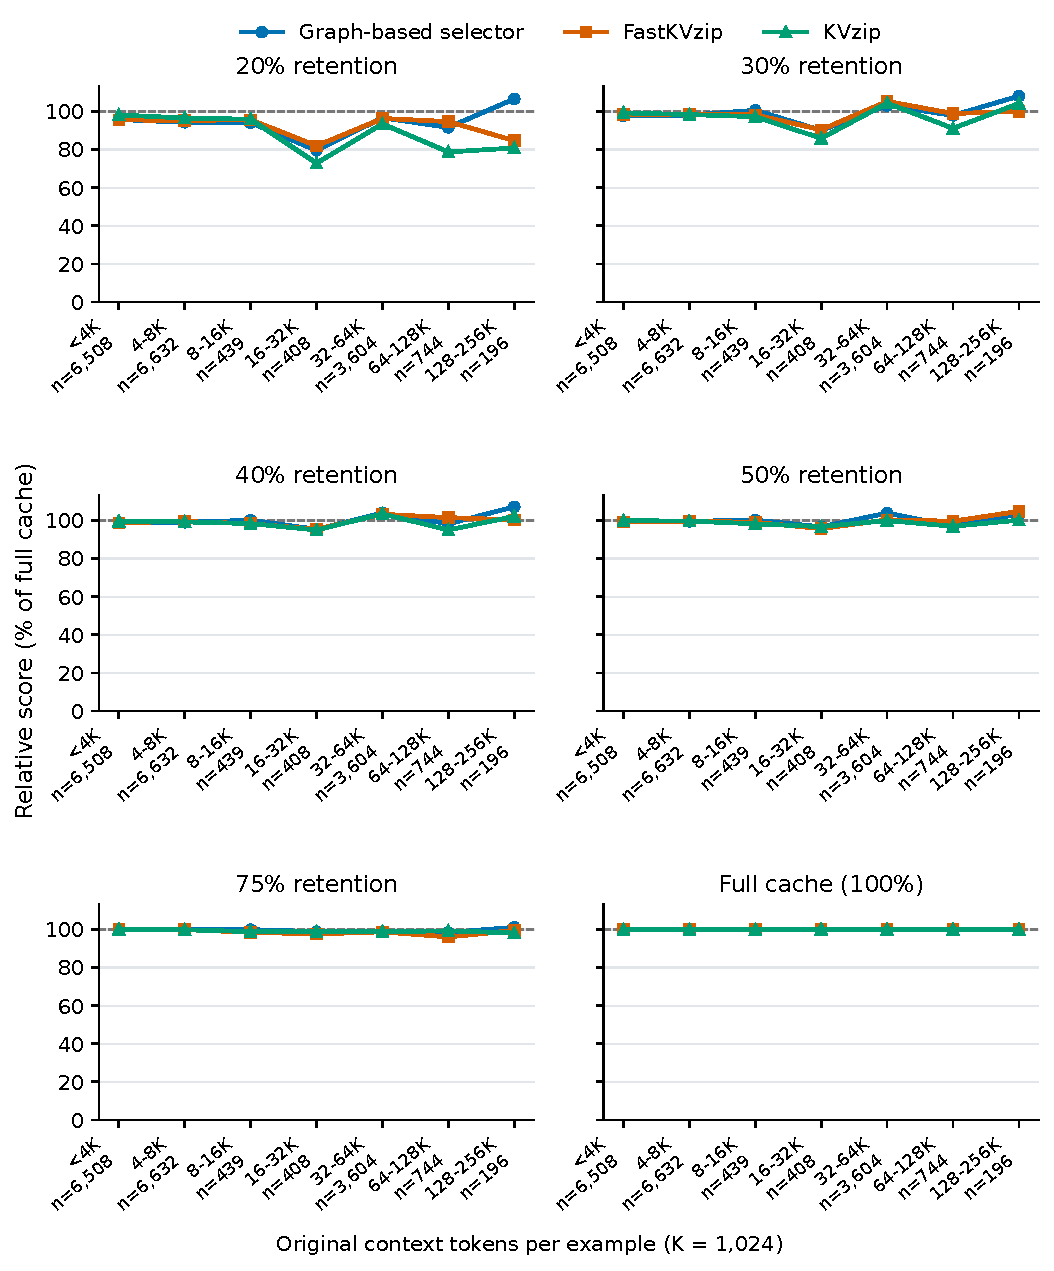
\includegraphics[width=\linewidth]{figures/context-score-buckets.pdf}
\caption{Full-cache-relative score by original context length, pooling all 18,531
matched context examples from the 60 evaluated RULER and SCBench
configurations. The same examples enter all three methods at every
retention ratio. Within each configuration and bucket, each method's mean
native-evaluator score is divided by its own full-cache mean on the same
contexts. These ratios are averaged with context-count weights and
multiplied by 100; no retention-ratio averaging is applied. All full-cache
denominators are positive. Dashed lines mark 100\% (full-cache performance);
values above 100\% indicate improvement over that baseline. Lengths are
measured before compression and exclude system, question, and chat-suffix
tokens. Buckets include their lower bound and exclude their upper bound;
K denotes 1,024 tokens, and $n$ is the number of contexts in a bucket.
Our selector and FastKVzip use a 2\% protected window; KVzip uses none.
The full-cache panel is 100\% by construction. Task composition
still varies across buckets, so the curves are descriptive rather
than a controlled context-length ablation.}
\label{fig:context-score-buckets}
\end{figure}

\clearpage
\section{Benchmark Guide and Evaluation Coverage}
\label{app:benchmarks}

The current report covers 60 of 107 configured variants. The remaining
47 need matched three-method results: 45 RULER, SQuAD, and
filtered GSM8K. This does not imply that they were never run in earlier
single-method experiments. LongBench v2, a later addition outside this
inventory, is described at the end of this appendix.

\paragraph{RULER.}
The 13 tasks in Table~\ref{tab:ruler-task-guide} cover retrieval, tracing,
aggregation, and question answering \citep{hsieh2024ruler}. We use the
standard 4K, 8K, 16K, 32K, 64K, and 128K context-length labels.
All tasks are reported at 4K and 8K; starred tasks are also reported at
64K. The other six 64K tasks and all 16K, 32K, and 128K tasks remain
outside the matched comparison.

\begin{table}[!ht]
\centering
\caption{RULER task descriptions \citep{hsieh2024ruler,nvidia2024rulerconfig}. Prefix identifiers with \texttt{ruler\_} and append the length label; $^{*}$ marks the seven tasks also reported at 64K.}
\label{tab:ruler-task-guide}
\small
\setlength{\tabcolsep}{4pt}
\renewcommand{\arraystretch}{1.18}
\begin{tabular}{@{}>{\raggedright\arraybackslash}p{1.20in}>{\raggedright\arraybackslash}p{4.13in}@{}}
\hline
Task & What it tests \\
\hline
\texttt{niah\_single\_1}$^{*}$ & Retrieve one numeric passkey associated with a word key, hidden among repetitive filler sentences. \\
\texttt{niah\_single\_2} & Retrieve one numeric passkey from natural-language essays instead of repetitive filler. \\
\texttt{niah\_single\_3} & Retrieve a UUID-valued needle from essays, testing exact recovery of a longer identifier. \\
\texttt{niah\_multikey\_1} & Choose the requested word--number association among four needles embedded in essays; three keys are distractors. \\
\texttt{niah\_multikey\_2} & Find a requested word--number association when the context is filled with competing key--value records. \\
\texttt{niah\_multikey\_3}$^{*}$ & Retrieve the UUID value for a UUID key from a dense collection of competing records. \\
\texttt{niah\_multivalue}$^{*}$ & Return all four numeric values associated with one key, distributed through an essay context. \\
\texttt{niah\_multiquery} & Answer four key lookups together, requiring recovery of every requested association from the context. \\
\texttt{vt}$^{*}$ & Follow a four-hop assignment chain and return the five variables that share the requested value. \\
\texttt{cwe}$^{*}$ & Recover ten unusually common words from a shuffled list; each target occurs more often than distractors. \\
\texttt{fwe}$^{*}$ & Identify the three most frequent words in a synthetic, skewed-frequency text, requiring global aggregation. \\
\texttt{qa\_1} & Answer a SQuAD-derived question using relevant passages surrounded by unrelated documents. \\
\texttt{qa\_2}$^{*}$ & Answer a HotpotQA-derived question with supporting passages and distractors, testing multi-hop evidence use. \\
\hline
\end{tabular}
\end{table}

Also remaining are \emph{SQuAD}, Wikipedia paragraph question answering
with roughly 160 context tokens, and \emph{GSM8K}, arithmetic word
problems with roughly 89 context tokens
\citep{rajpurkar2016squad,cobbe2021gsm8k}. Our SQuAD adapter uses the
training split (18,891 contexts); GSM retains 148 test examples with at
least 72 context tokens. Neither is the full official held-out evaluation.

\clearpage
\paragraph{SCBench.}
SCBench asks multiple questions about a shared context \citep{li2025scbench}.
Table~\ref{tab:scbench-task-guide} combines task descriptions with average
context lengths for every prepared variant, using
\href{https://huggingface.co/datasets/Jang-Hyun/SCBench-preprocessed}{\texttt{SCBench-preprocessed}}
as in KVzip \citep{kim2025kvzip}.
All 11 base tasks and 16 prepared length variants now have matched results
for all three methods.

\begin{table}[!ht]
\centering
\caption{SCBench tasks and average raw-context Qwen tokens, rounded to the nearest thousand (K). Add \texttt{scbench\_} to each task and the listed suffix for a variant; \emph{base} has no suffix. All 27 variants are in the current report. System, question, and chat-suffix tokens are excluded.}
\label{tab:scbench-task-guide}
\small
\setlength{\tabcolsep}{4pt}
\renewcommand{\arraystretch}{1.15}
\begin{tabular}{@{}>{\raggedright\arraybackslash}p{1.45in}>{\raggedright\arraybackslash}p{0.92in}>{\raggedright\arraybackslash}p{2.85in}@{}}
\hline
Task & Avg. tokens & What it tests \\
\hline
\texttt{kv} & base 169K\newline mid 85K\newline short 25K\newline tiny 11K & Retrieve the value for a requested key from a large dictionary of random key--value records. \\
\texttt{mf} & base 145K\newline mid 73K\newline short 29K\newline tiny 12K & Find requested numerical statistics, such as extrema or the median, in a long array. \\
\texttt{qa\_eng} & base 92K & Answer free-form English questions about a long narrative, locating the relevant evidence in the text. \\
\texttt{repoqa} & base 67K\newline short 15K\newline tiny 7K & Return the repository function matching a natural-language description, testing semantic code retrieval. \\
\texttt{summary} & base 105K\newline mid 13K\newline short 13K\newline tiny 12K & Summarize a requested paper within a concatenation of academic papers, ignoring the other documents. \\
\texttt{choice\_eng} & base 95K & Select the correct multiple-choice answer to a question about a long English narrative. \\
\texttt{many\_shot} & base 24K\newline short 15K\newline tiny 8K & Infer tasks from many demonstrations, including date understanding, translation-error detection, and shuffled-object tracking. \\
\texttt{prefix\_suffix} & base 112K\newline mid 56K\newline short 19K\newline tiny 8K & Recover a dictionary string matching both a supplied prefix and suffix, despite partial-match distractors. \\
\texttt{vt} & base 125K & Track variable assignments through a noisy context and identify variables sharing a requested value. \\
\texttt{summary\_with\_needles} & base 105K & Use one context for both document summarization and retrieval of inserted passkeys. \\
\texttt{repoqa\_and\_kv} & base 70K & Alternate semantic function retrieval and exact key--value lookup within a shared repository context. \\
\hline
\end{tabular}
\end{table}

\paragraph{LongBench v2.}
LongBench v2 \citep{bai2024longbenchv2} contains 503 four-way
multiple-choice questions, written and verified by human annotators, over
realistic long-context material: single-document QA, multi-document QA, long
in-context learning, long-dialogue history understanding, code-repository
understanding, and long structured-data understanding, with contexts from 8K
to 2M words. It is a single configuration, evaluated in full on all 503
questions for all three methods and reported in
Section~\ref{sec:main-results}. Contexts longer than the model's 1M-token
limit are truncated, the model answers directly without chain-of-thought, and
the score is exact-match accuracy over the 503 questions.

\clearpage
% Generated by plot_retention_scores.py; edit the generator instead.
\section{Retention--Score Curves}
\label{app:retention-curves}

This appendix plots all 60 matched configurations and their benchmark and task-family summaries. The seven benchmark summaries reproduce the aggregate rows in Tables~\ref{tab:results-graphkv}--\ref{tab:results-kvzip}. Each aggregate is the arithmetic mean of its unrounded configuration scores, independently at each retention ratio. All plots use absolute native-evaluator scores (0--100) and the same method colors. Each panel has a zoomed linear y-axis enclosing all three methods and their full-cache baselines. Y-axis ranges vary across panels; tick labels show the actual scores. Flat and near-flat panels span at least two score points, and identical constant curves are explicitly marked.

Solid curves show the three methods at 20, 30, 40, 50, 75, and 100\% retention. 17 of 98 panels additionally include 5 and 10\% retention: the 11 SCBench base tasks, their aggregate mean, and their four family panels. These two extra points were evaluated only for the 11 SCBench base tasks; the 16 length variants and all RULER configurations are unaffected and still span 20--100\%. Dashed horizontal lines show each method's own measured full-cache score, using the matching color; one gray dashed line is used when all three full-cache scores coincide. Coincident curves and nearly equal baselines may overlap. The full-cache point is included at 100\% retention. SCBench base-task and all-variant means are distinguished; RULER 64K contains only seven selected tasks.

SCBench families follow Section~3.1 and Table~2 of \citet{li2025scbench}: string retrieval, semantic retrieval, global information processing, and multi-tasking. Chinese QA is absent from our semantic-retrieval subset. Prepared length variants inherit their base task's family. RULER families and needle-retrieval subtypes follow Section~3 of \citet{hsieh2024ruler}. One-task families repeat their individual curve for convenient comparison. The deployed combined scores for mixed SCBench and Many-shot tasks are retained; component scores are not separately available in the table snapshot. Unevaluated configurations have no curves.

\paragraph{Plot guide.}
Benchmark summaries (Figures~\ref{fig:retention-suite-overview}--\ref{fig:retention-ruler-lengths}); SCBench task families (Figures~\ref{fig:retention-scbench-families-base-tasks}--\ref{fig:retention-scbench-families-all-variants}); RULER task families (Figures~\ref{fig:retention-ruler-4k}--\ref{fig:retention-ruler-64k}); RULER retrieval subtypes (Figures~\ref{fig:retention-ruler-retrieval-subtypes-4k}--\ref{fig:retention-ruler-retrieval-subtypes-64k}); SCBench individual tasks (Figures~\ref{fig:retention-scbench-tasks-1}--\ref{fig:retention-scbench-tasks-5}); RULER 4K individual tasks (Figures~\ref{fig:retention-ruler-4k-tasks-1}--\ref{fig:retention-ruler-4k-tasks-3}); RULER 8K individual tasks (Figures~\ref{fig:retention-ruler-8k-tasks-1}--\ref{fig:retention-ruler-8k-tasks-3}); RULER 64K individual tasks (Figures~\ref{fig:retention-ruler-64k-tasks-1}--\ref{fig:retention-ruler-64k-tasks-2}).
\clearpage

\subsection{Benchmark summaries}

\begin{figure}[!ht]
\centering
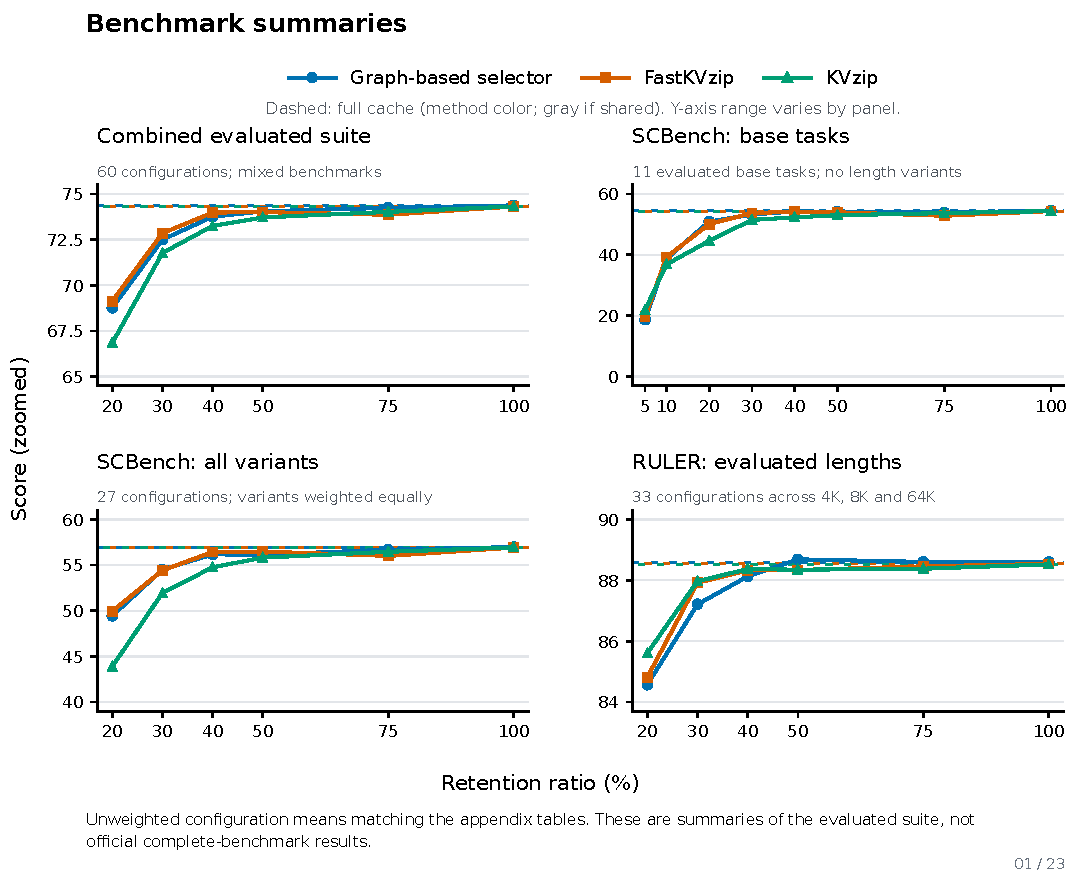
\includegraphics[width=\linewidth]{figures/retention-curves/01-suite-overview.pdf}
\caption{Benchmark summaries.}
\label{fig:retention-suite-overview}
\end{figure}
\clearpage

\begin{figure}[!ht]
\centering
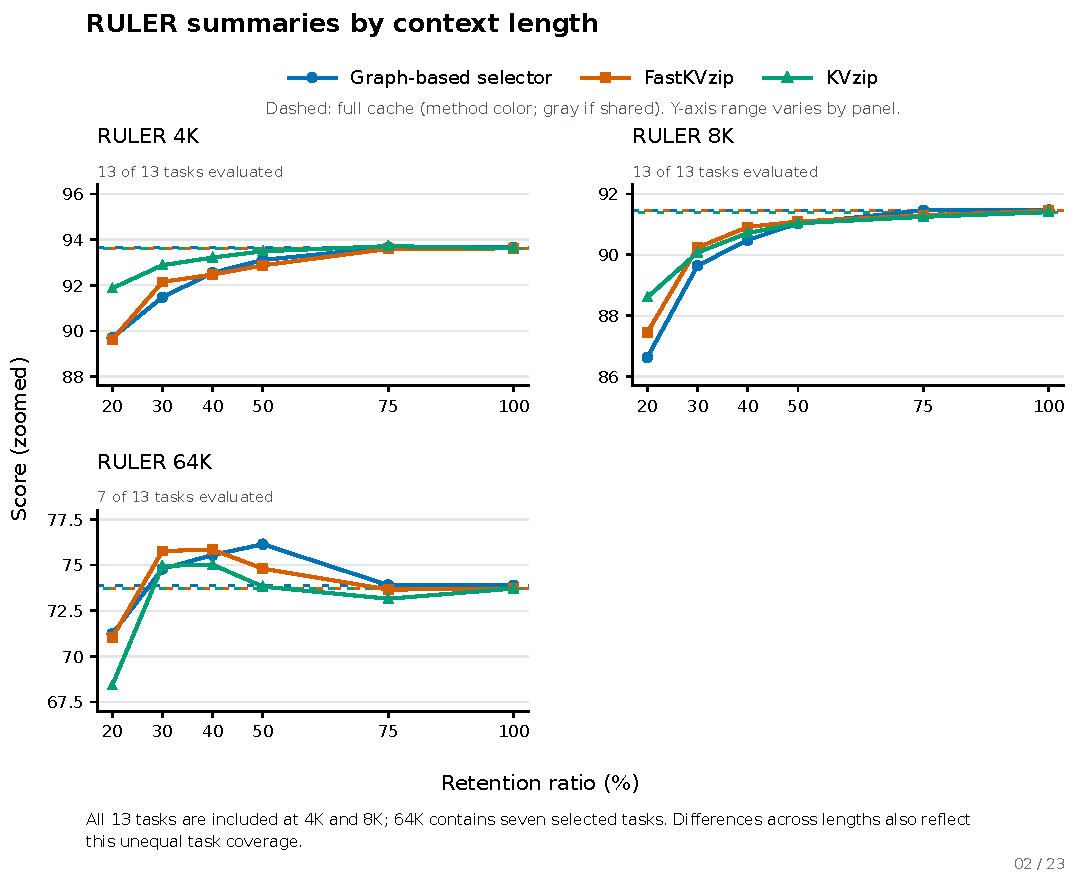
\includegraphics[width=\linewidth]{figures/retention-curves/02-ruler-lengths.pdf}
\caption{RULER summaries by context length.}
\label{fig:retention-ruler-lengths}
\end{figure}
\clearpage

\subsection{SCBench task families}

\begin{figure}[!ht]
\centering
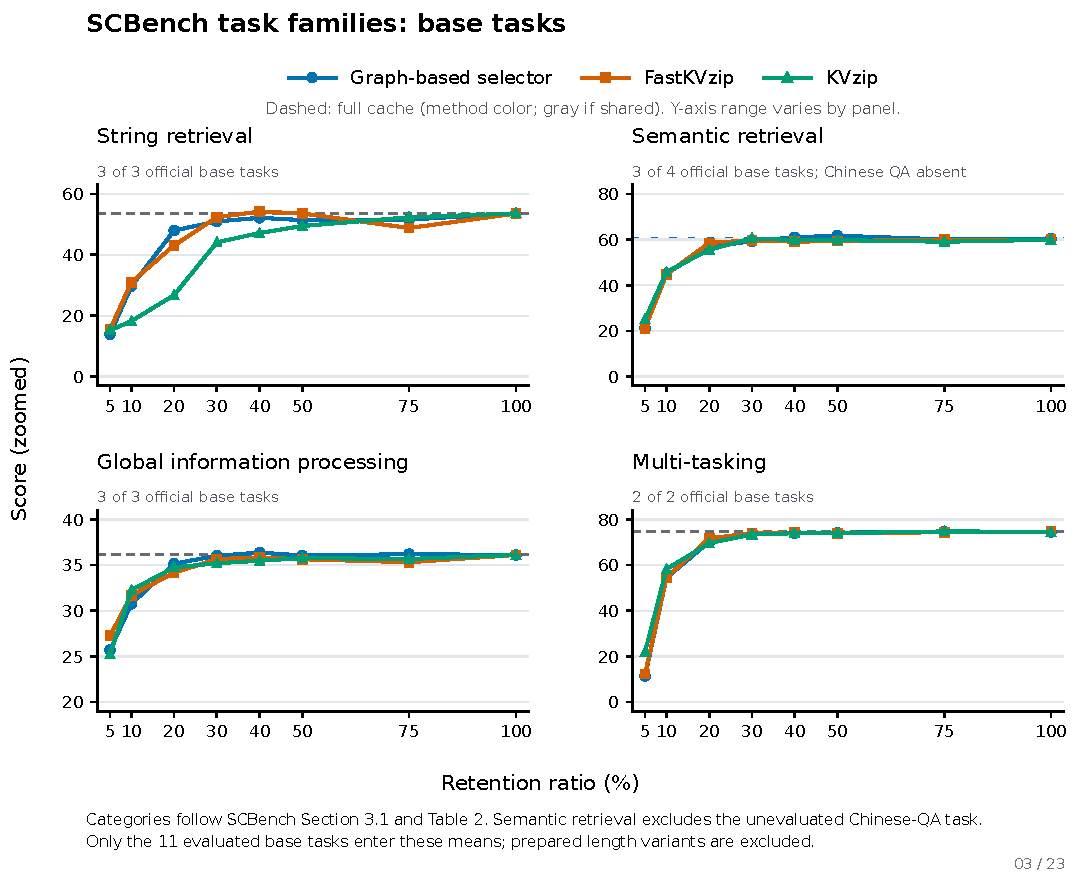
\includegraphics[width=\linewidth]{figures/retention-curves/03-scbench-families-base-tasks.pdf}
\caption{SCBench task families: base tasks.}
\label{fig:retention-scbench-families-base-tasks}
\end{figure}
\clearpage

\begin{figure}[!ht]
\centering
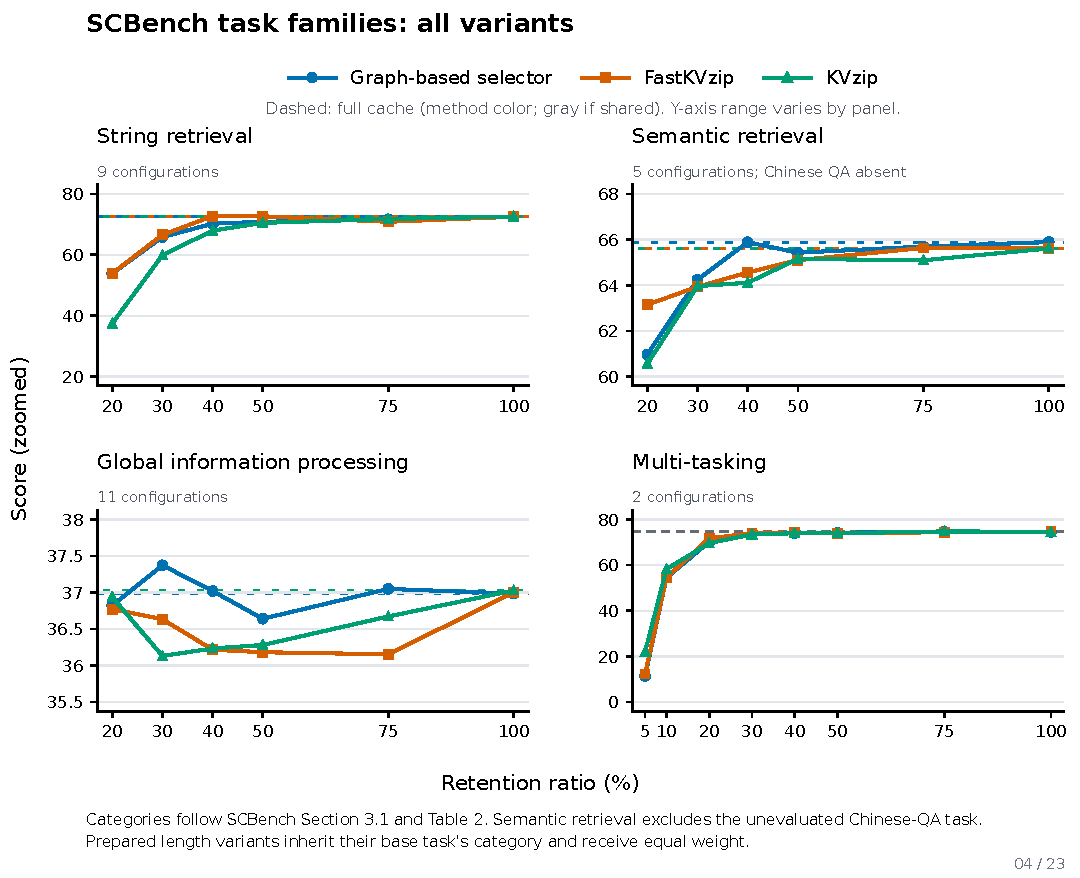
\includegraphics[width=\linewidth]{figures/retention-curves/04-scbench-families-all-variants.pdf}
\caption{SCBench task families: all variants.}
\label{fig:retention-scbench-families-all-variants}
\end{figure}
\clearpage

\subsection{RULER task families}

\begin{figure}[!ht]
\centering
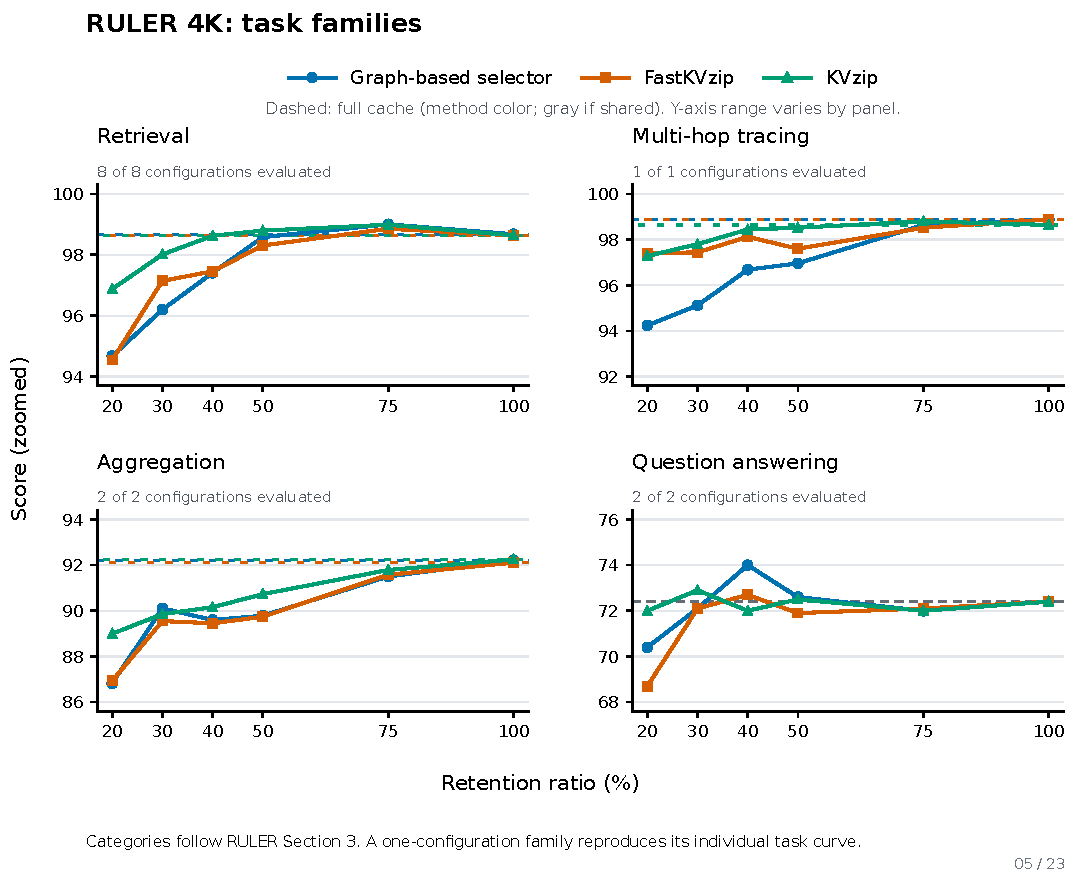
\includegraphics[width=\linewidth]{figures/retention-curves/05-ruler-4k.pdf}
\caption{RULER 4K: task families.}
\label{fig:retention-ruler-4k}
\end{figure}
\clearpage

\begin{figure}[!ht]
\centering
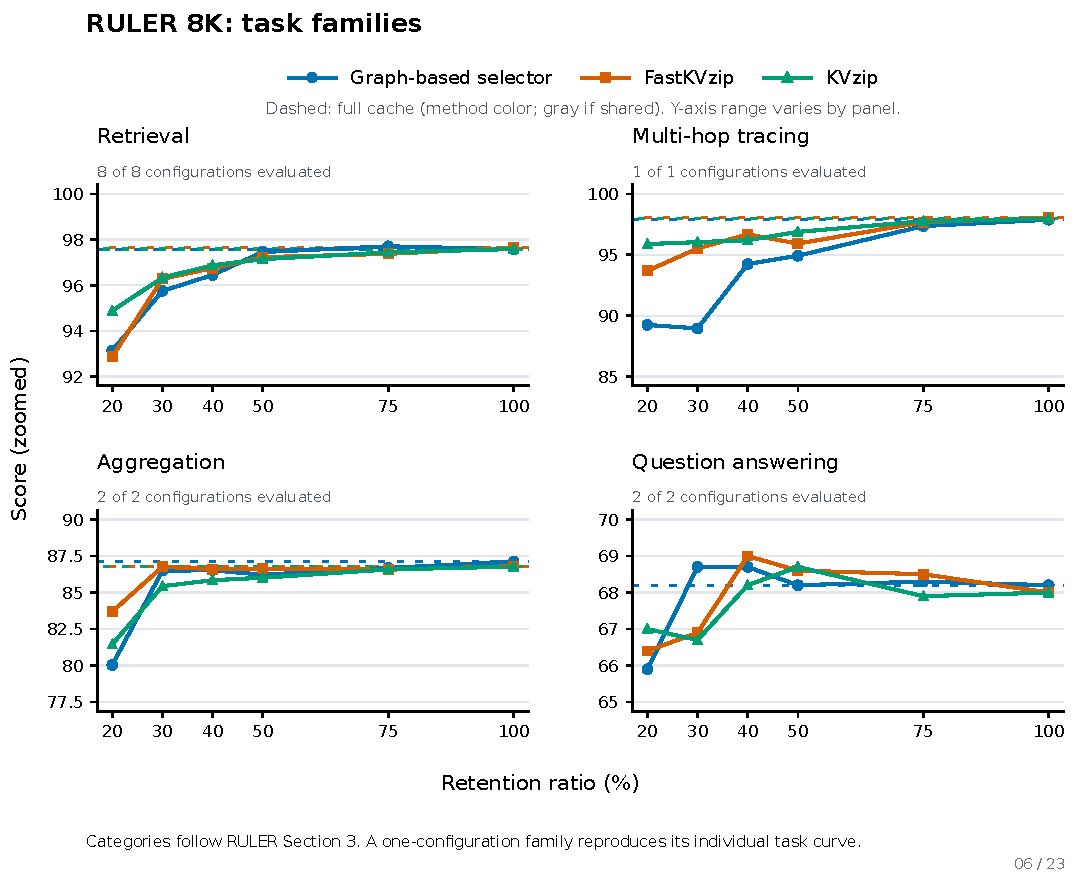
\includegraphics[width=\linewidth]{figures/retention-curves/06-ruler-8k.pdf}
\caption{RULER 8K: task families.}
\label{fig:retention-ruler-8k}
\end{figure}
\clearpage

\begin{figure}[!ht]
\centering
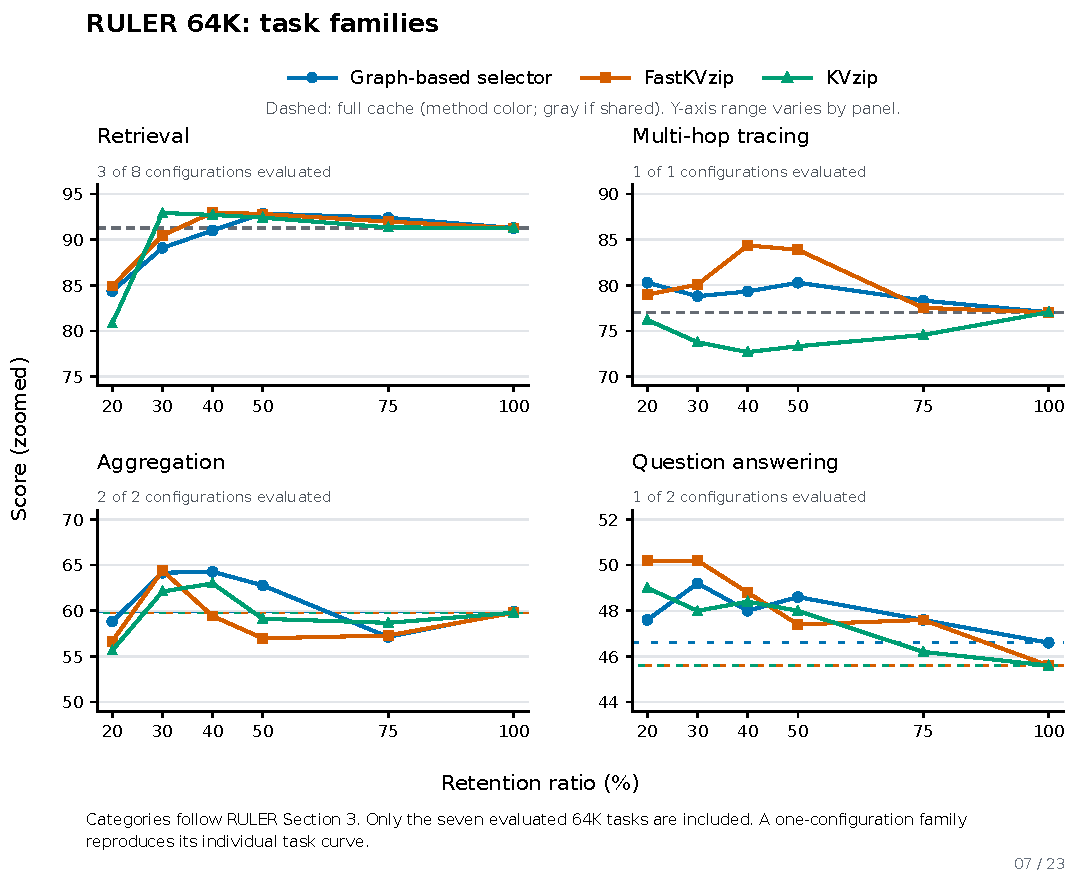
\includegraphics[width=\linewidth]{figures/retention-curves/07-ruler-64k.pdf}
\caption{RULER 64K: task families.}
\label{fig:retention-ruler-64k}
\end{figure}
\clearpage

\subsection{RULER retrieval subtypes}

\begin{figure}[!ht]
\centering
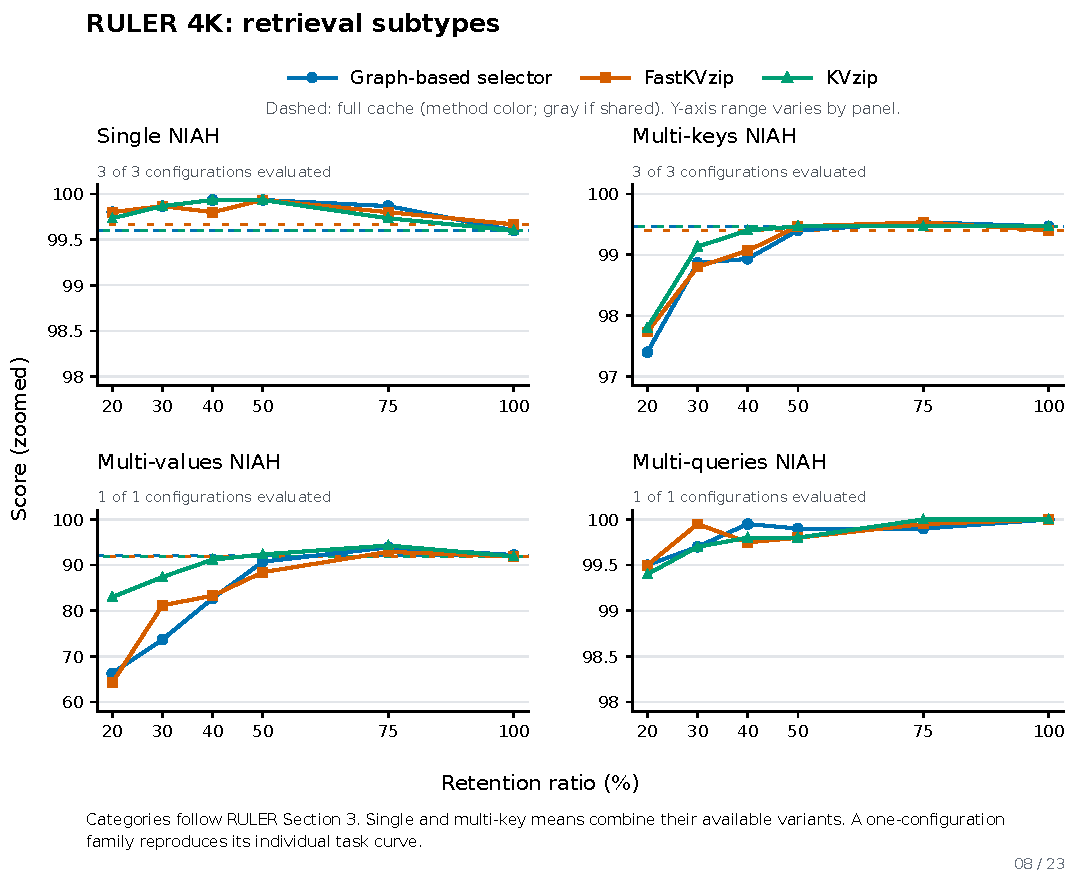
\includegraphics[width=\linewidth]{figures/retention-curves/08-ruler-retrieval-subtypes-4k.pdf}
\caption{RULER 4K: retrieval subtypes.}
\label{fig:retention-ruler-retrieval-subtypes-4k}
\end{figure}
\clearpage

\begin{figure}[!ht]
\centering
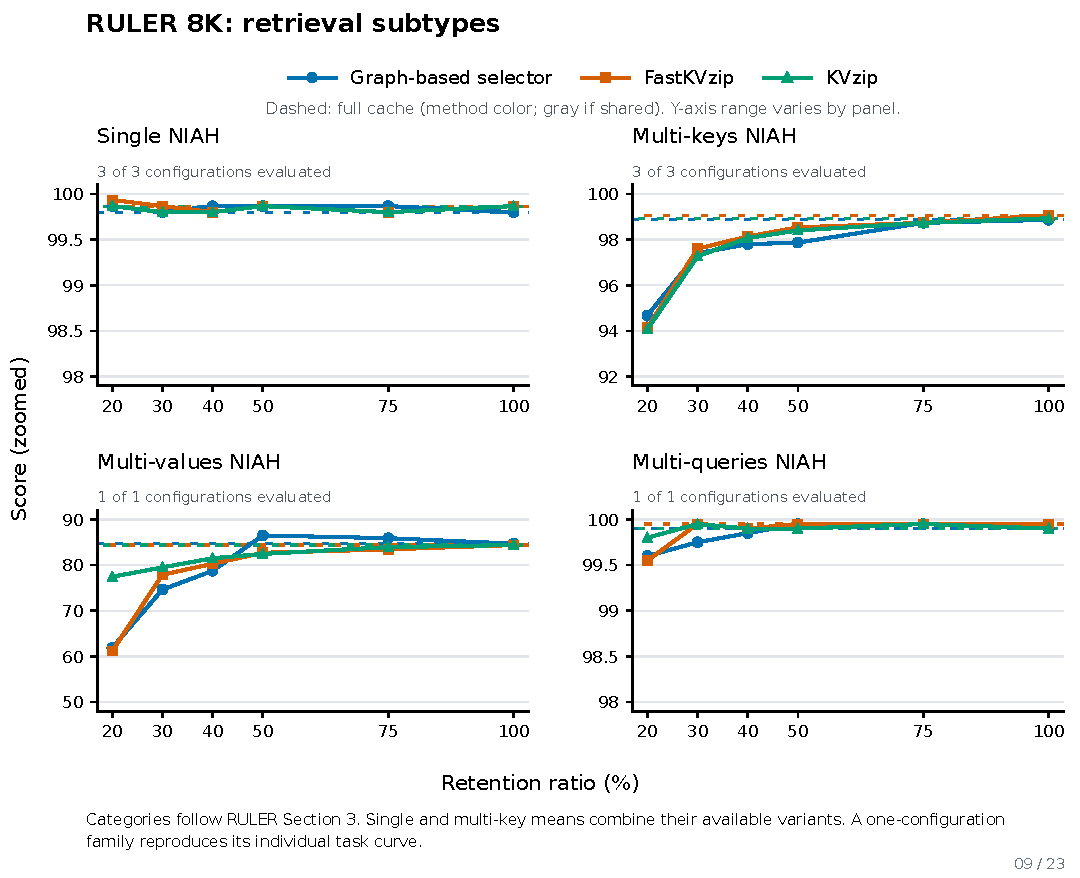
\includegraphics[width=\linewidth]{figures/retention-curves/09-ruler-retrieval-subtypes-8k.pdf}
\caption{RULER 8K: retrieval subtypes.}
\label{fig:retention-ruler-retrieval-subtypes-8k}
\end{figure}
\clearpage

\begin{figure}[!ht]
\centering
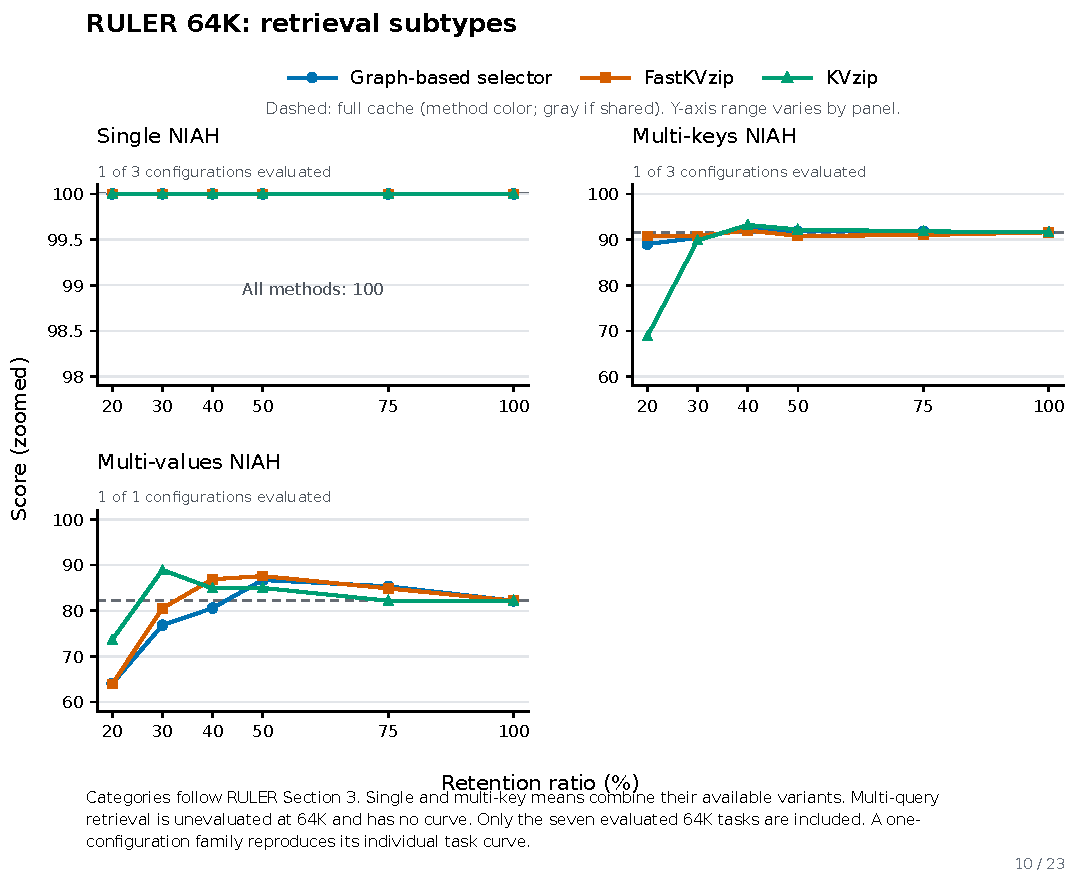
\includegraphics[width=\linewidth]{figures/retention-curves/10-ruler-retrieval-subtypes-64k.pdf}
\caption{RULER 64K: retrieval subtypes.}
\label{fig:retention-ruler-retrieval-subtypes-64k}
\end{figure}
\clearpage

\subsection{SCBench individual tasks}

\begin{figure}[!ht]
\centering
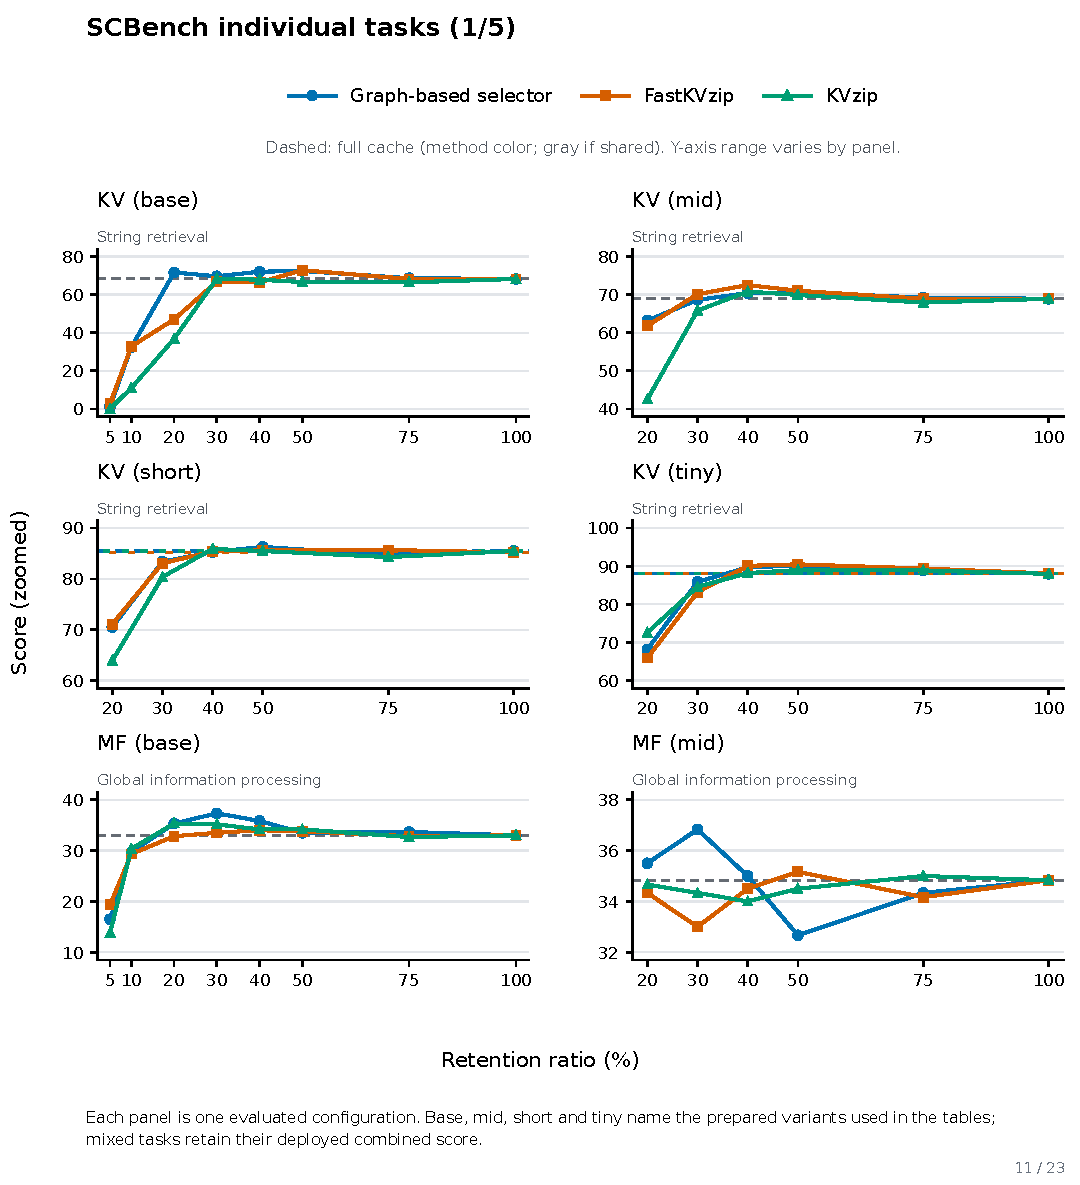
\includegraphics[width=\linewidth]{figures/retention-curves/11-scbench-tasks-1.pdf}
\caption{SCBench individual tasks (1/5).}
\label{fig:retention-scbench-tasks-1}
\end{figure}
\clearpage

\begin{figure}[!ht]
\centering
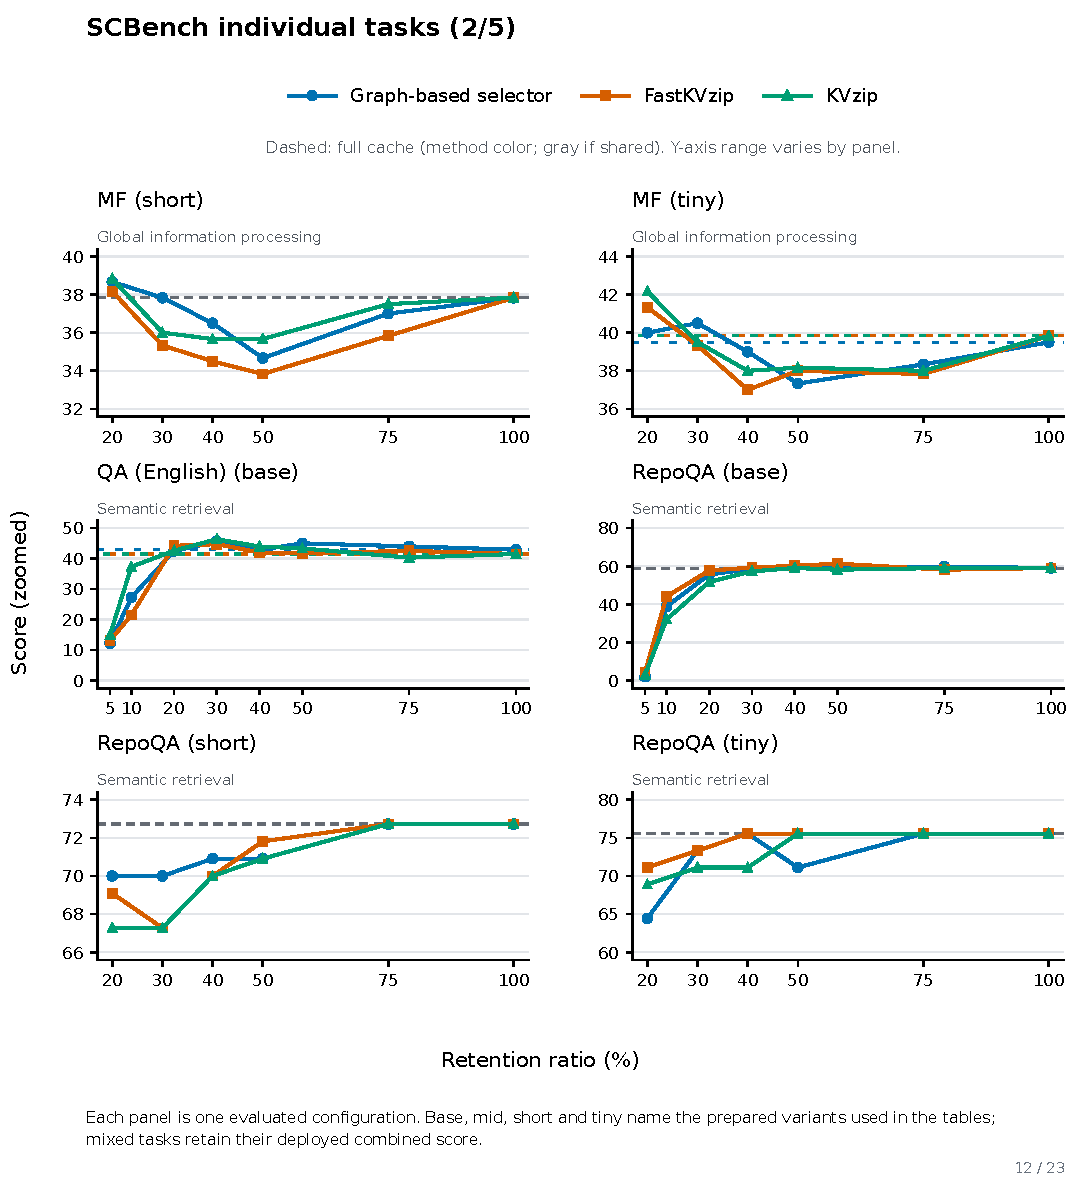
\includegraphics[width=\linewidth]{figures/retention-curves/12-scbench-tasks-2.pdf}
\caption{SCBench individual tasks (2/5).}
\label{fig:retention-scbench-tasks-2}
\end{figure}
\clearpage

\begin{figure}[!ht]
\centering
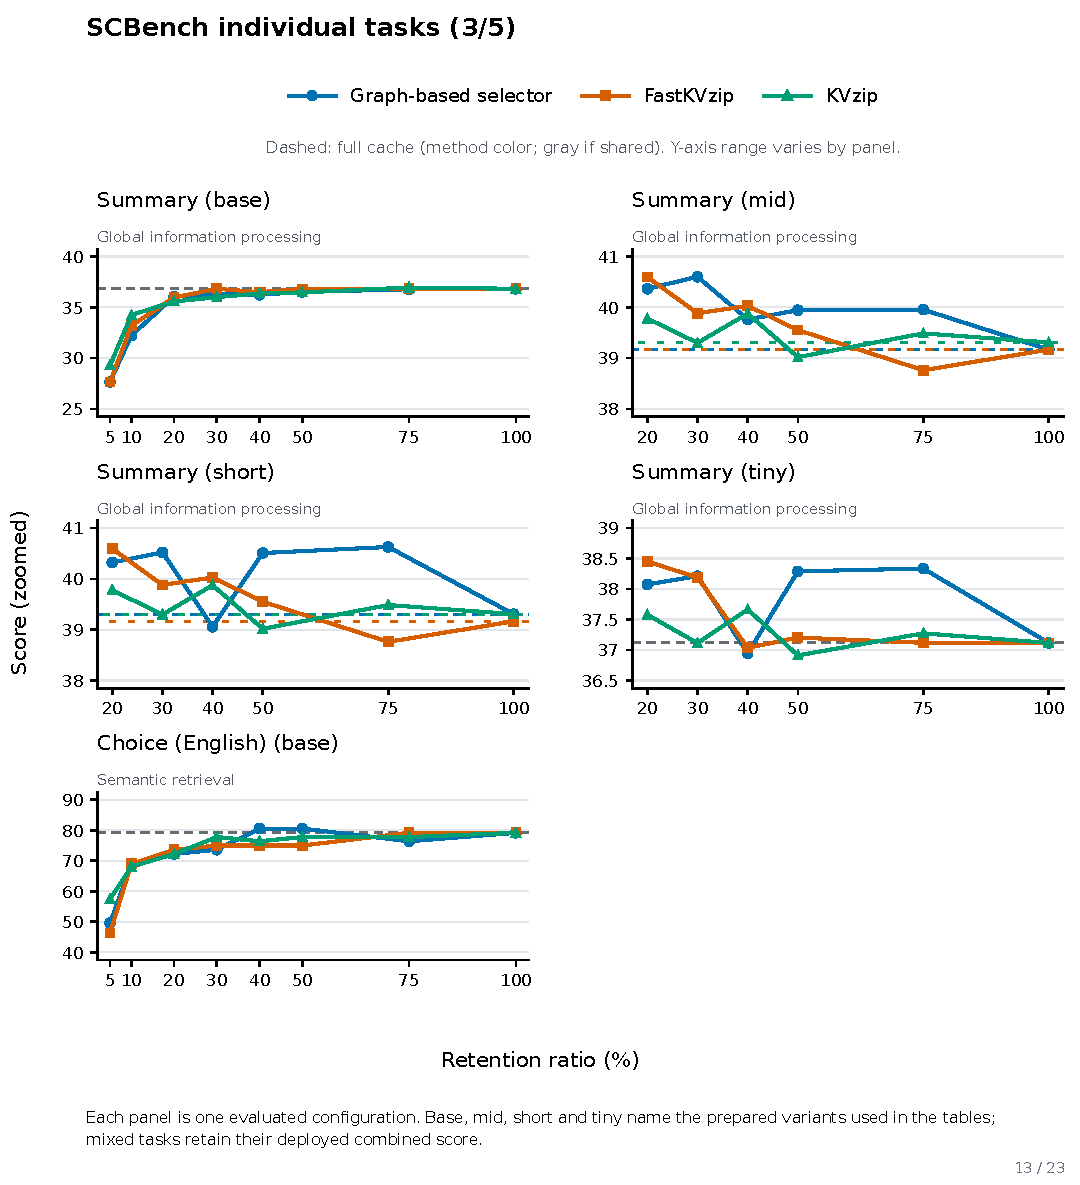
\includegraphics[width=\linewidth]{figures/retention-curves/13-scbench-tasks-3.pdf}
\caption{SCBench individual tasks (3/5).}
\label{fig:retention-scbench-tasks-3}
\end{figure}
\clearpage

\begin{figure}[!ht]
\centering
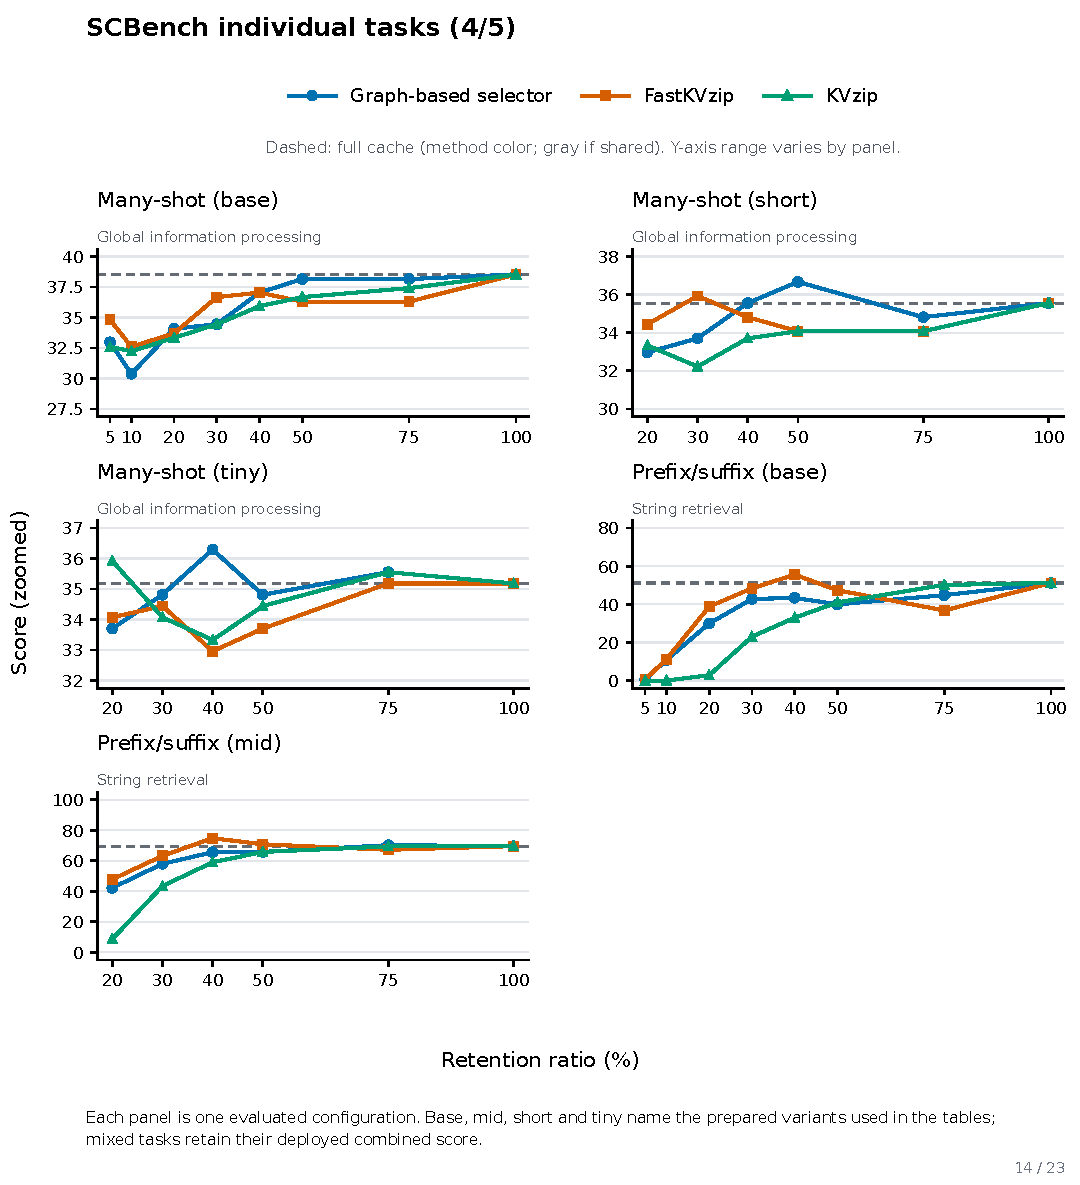
\includegraphics[width=\linewidth]{figures/retention-curves/14-scbench-tasks-4.pdf}
\caption{SCBench individual tasks (4/5).}
\label{fig:retention-scbench-tasks-4}
\end{figure}
\clearpage

\begin{figure}[!ht]
\centering
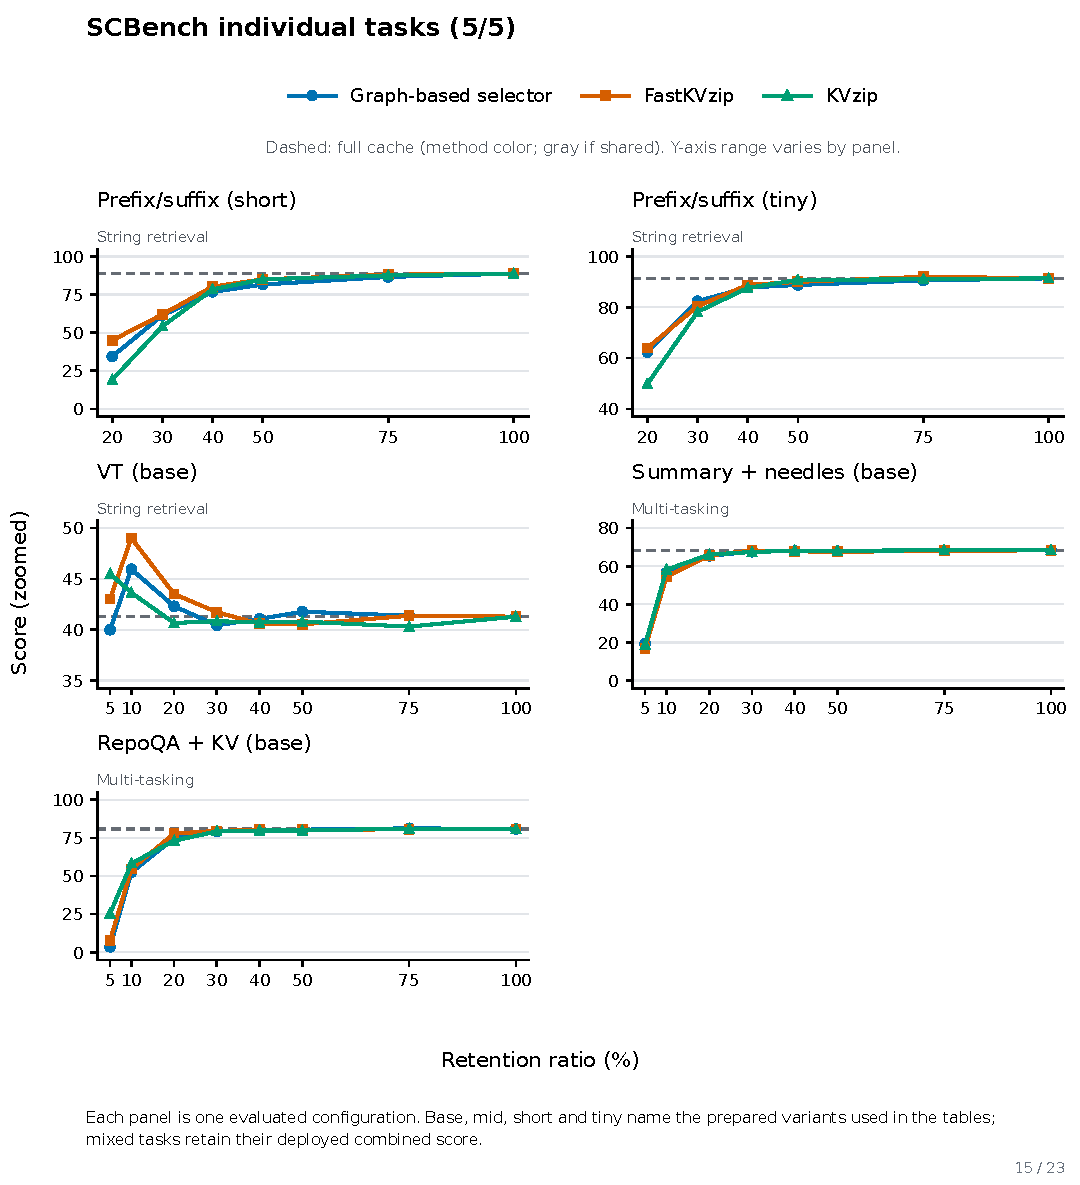
\includegraphics[width=\linewidth]{figures/retention-curves/15-scbench-tasks-5.pdf}
\caption{SCBench individual tasks (5/5).}
\label{fig:retention-scbench-tasks-5}
\end{figure}
\clearpage

\subsection{RULER 4K individual tasks}

\begin{figure}[!ht]
\centering
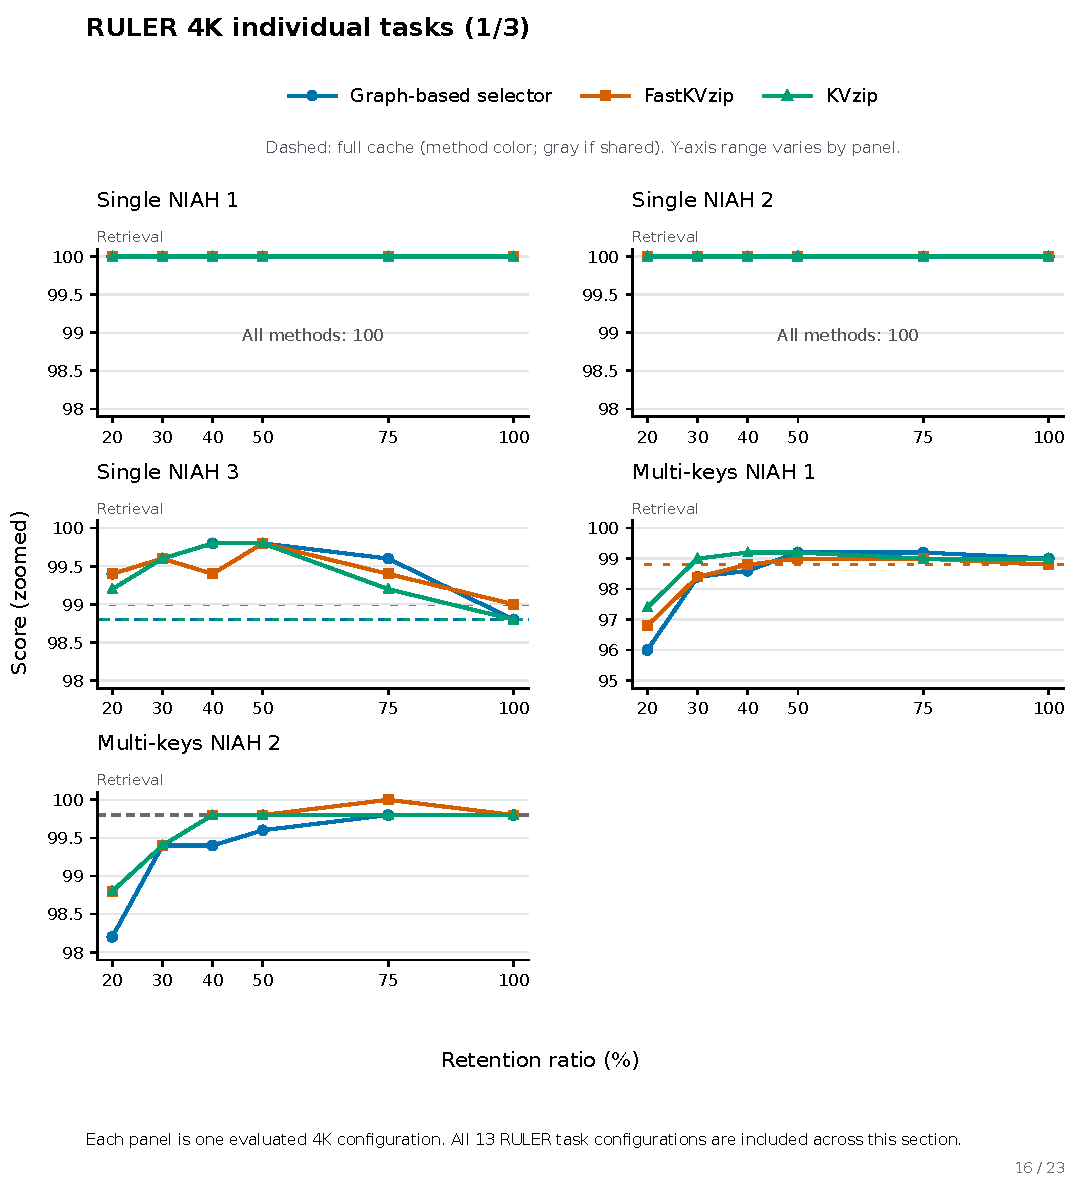
\includegraphics[width=\linewidth]{figures/retention-curves/16-ruler-4k-tasks-1.pdf}
\caption{RULER 4K individual tasks (1/3).}
\label{fig:retention-ruler-4k-tasks-1}
\end{figure}
\clearpage

\begin{figure}[!ht]
\centering
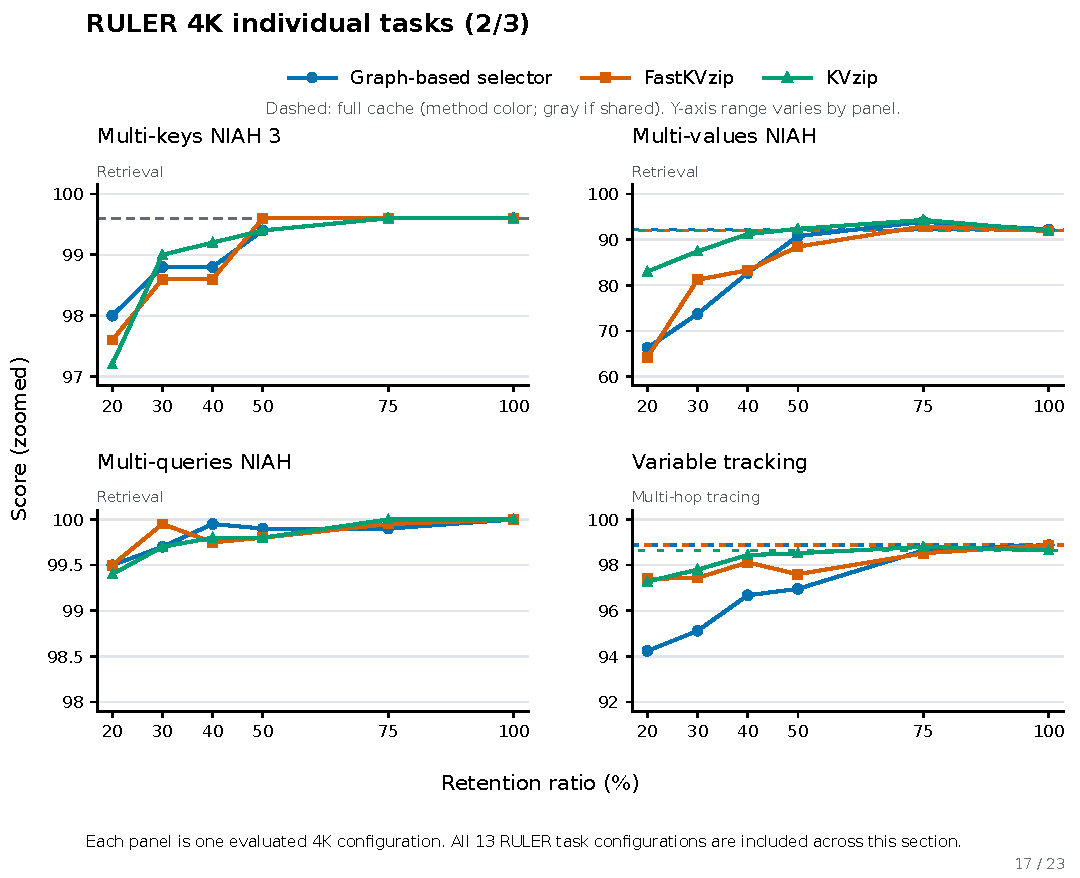
\includegraphics[width=\linewidth]{figures/retention-curves/17-ruler-4k-tasks-2.pdf}
\caption{RULER 4K individual tasks (2/3).}
\label{fig:retention-ruler-4k-tasks-2}
\end{figure}
\clearpage

\begin{figure}[!ht]
\centering
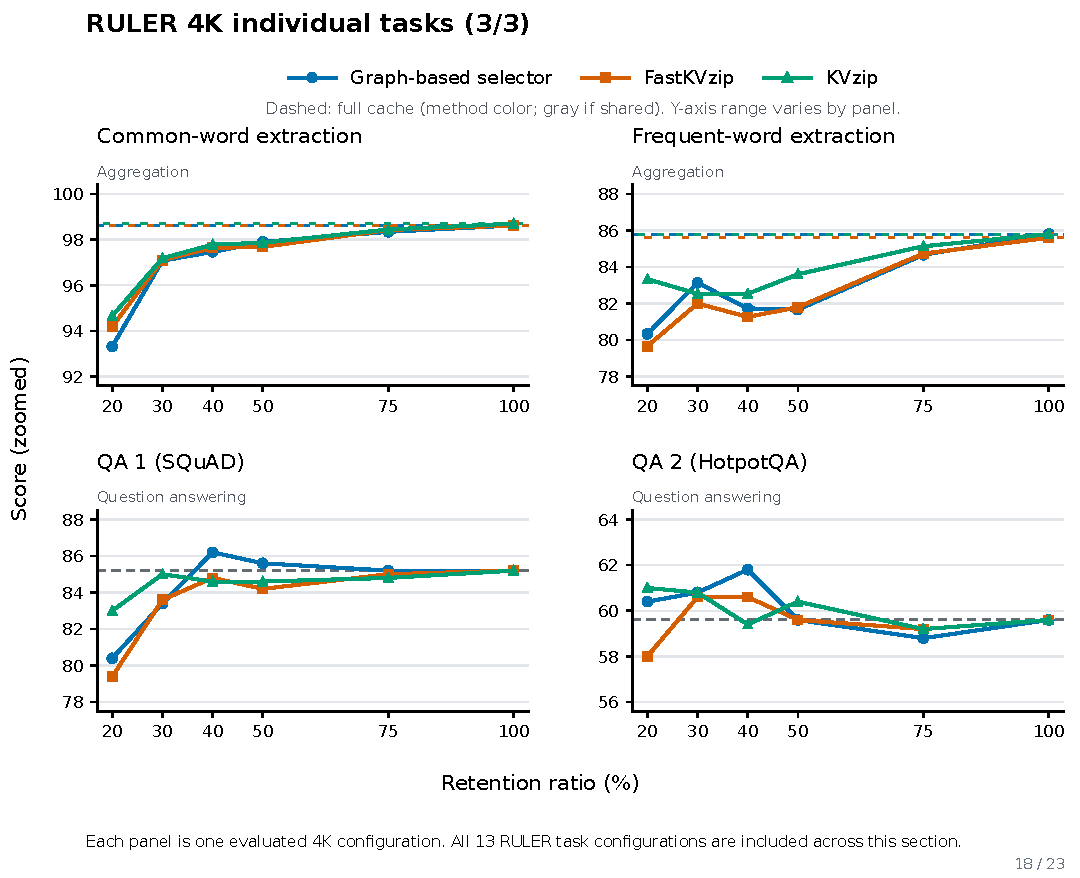
\includegraphics[width=\linewidth]{figures/retention-curves/18-ruler-4k-tasks-3.pdf}
\caption{RULER 4K individual tasks (3/3).}
\label{fig:retention-ruler-4k-tasks-3}
\end{figure}
\clearpage

\subsection{RULER 8K individual tasks}

\begin{figure}[!ht]
\centering
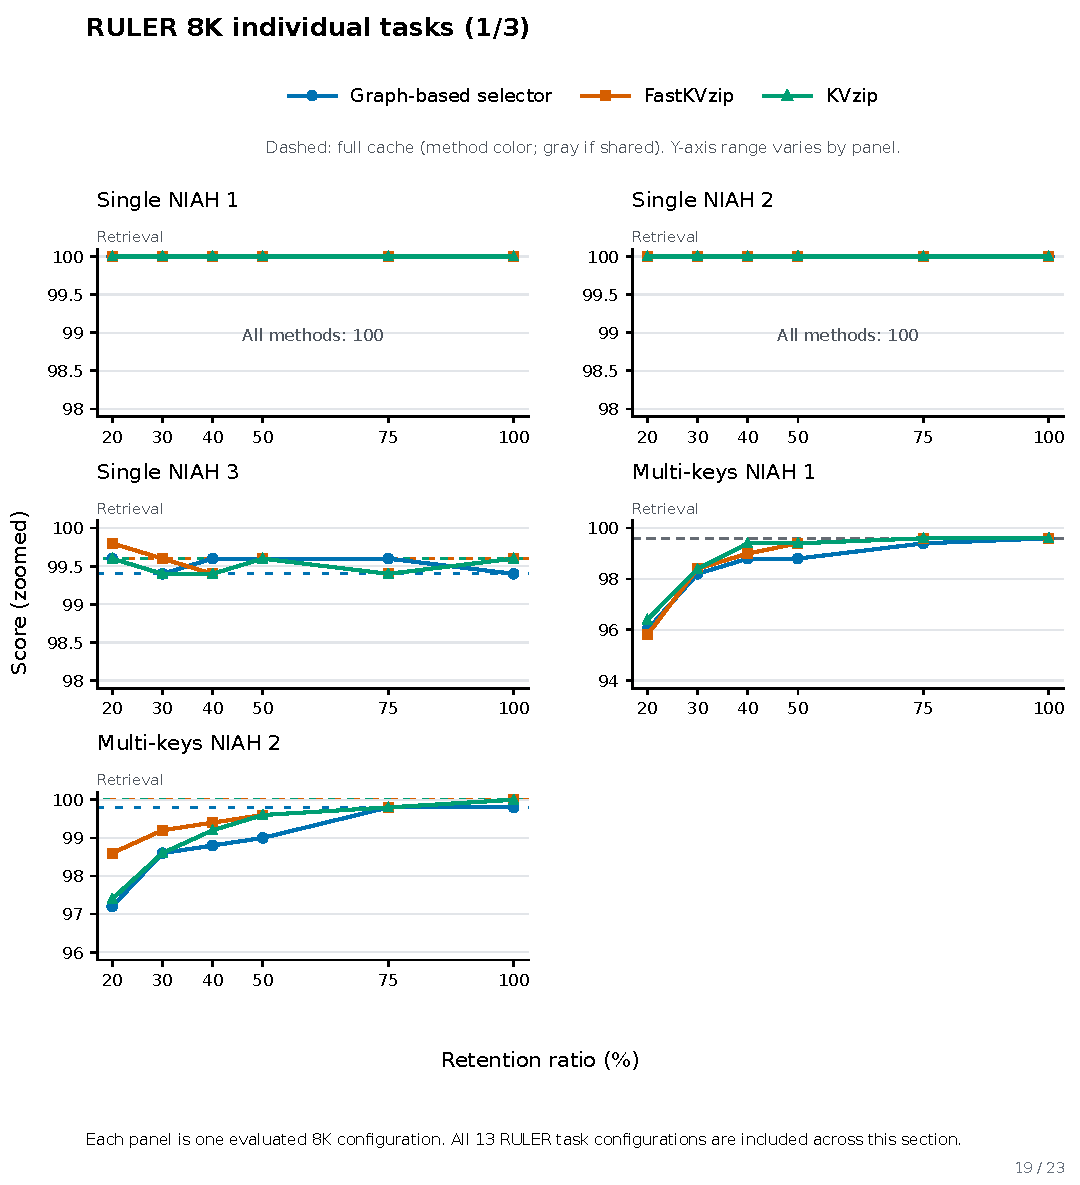
\includegraphics[width=\linewidth]{figures/retention-curves/19-ruler-8k-tasks-1.pdf}
\caption{RULER 8K individual tasks (1/3).}
\label{fig:retention-ruler-8k-tasks-1}
\end{figure}
\clearpage

\begin{figure}[!ht]
\centering
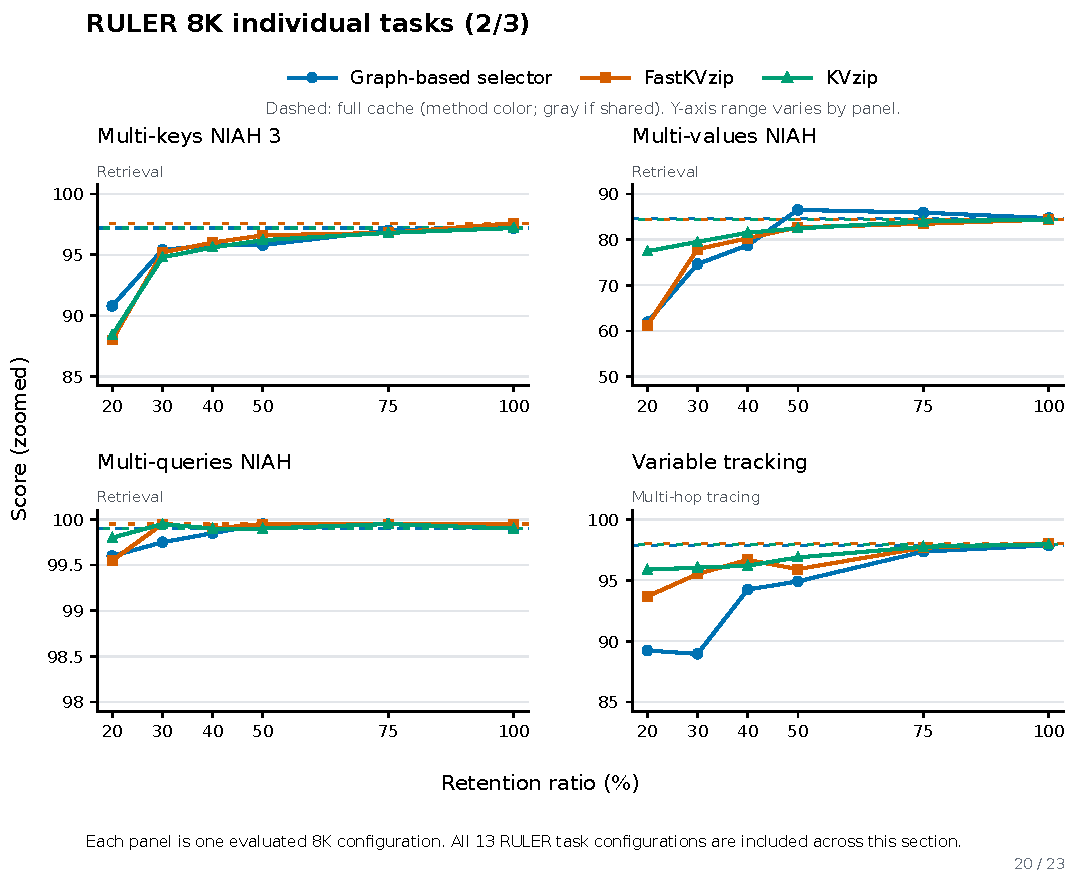
\includegraphics[width=\linewidth]{figures/retention-curves/20-ruler-8k-tasks-2.pdf}
\caption{RULER 8K individual tasks (2/3).}
\label{fig:retention-ruler-8k-tasks-2}
\end{figure}
\clearpage

\begin{figure}[!ht]
\centering
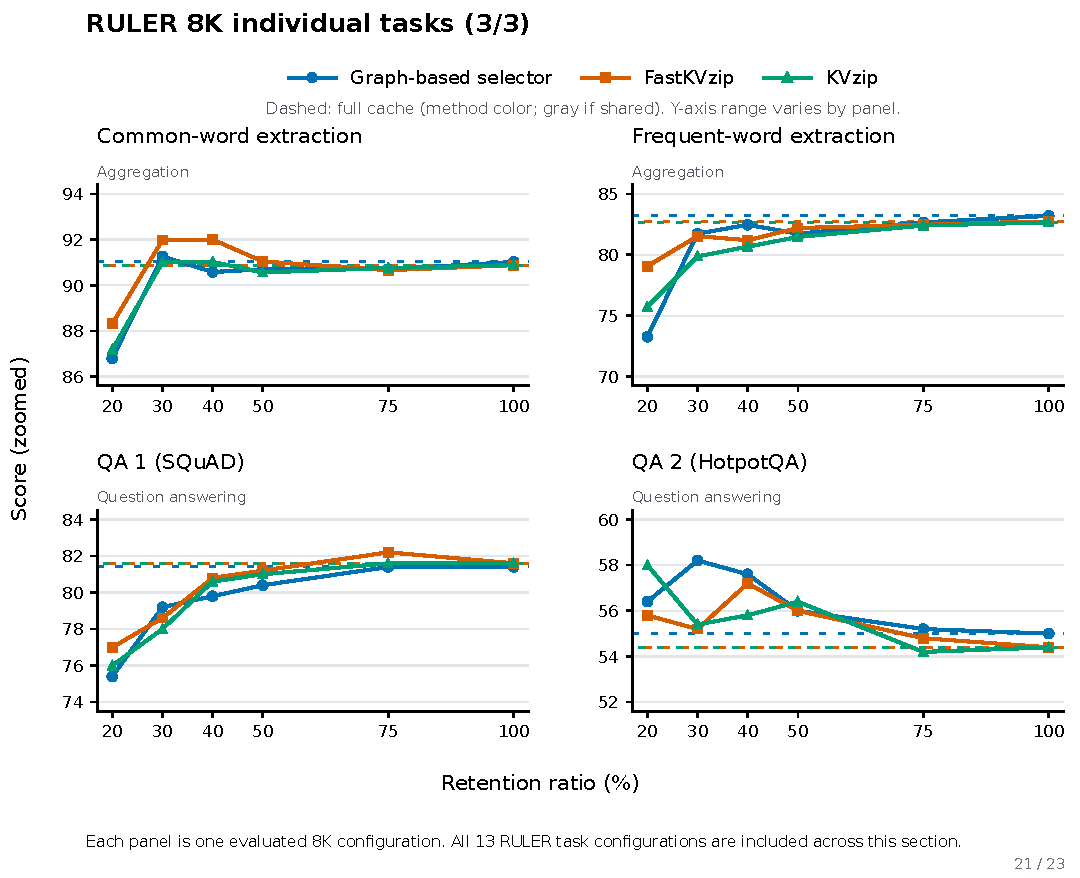
\includegraphics[width=\linewidth]{figures/retention-curves/21-ruler-8k-tasks-3.pdf}
\caption{RULER 8K individual tasks (3/3).}
\label{fig:retention-ruler-8k-tasks-3}
\end{figure}
\clearpage

\subsection{RULER 64K individual tasks}

\begin{figure}[!ht]
\centering
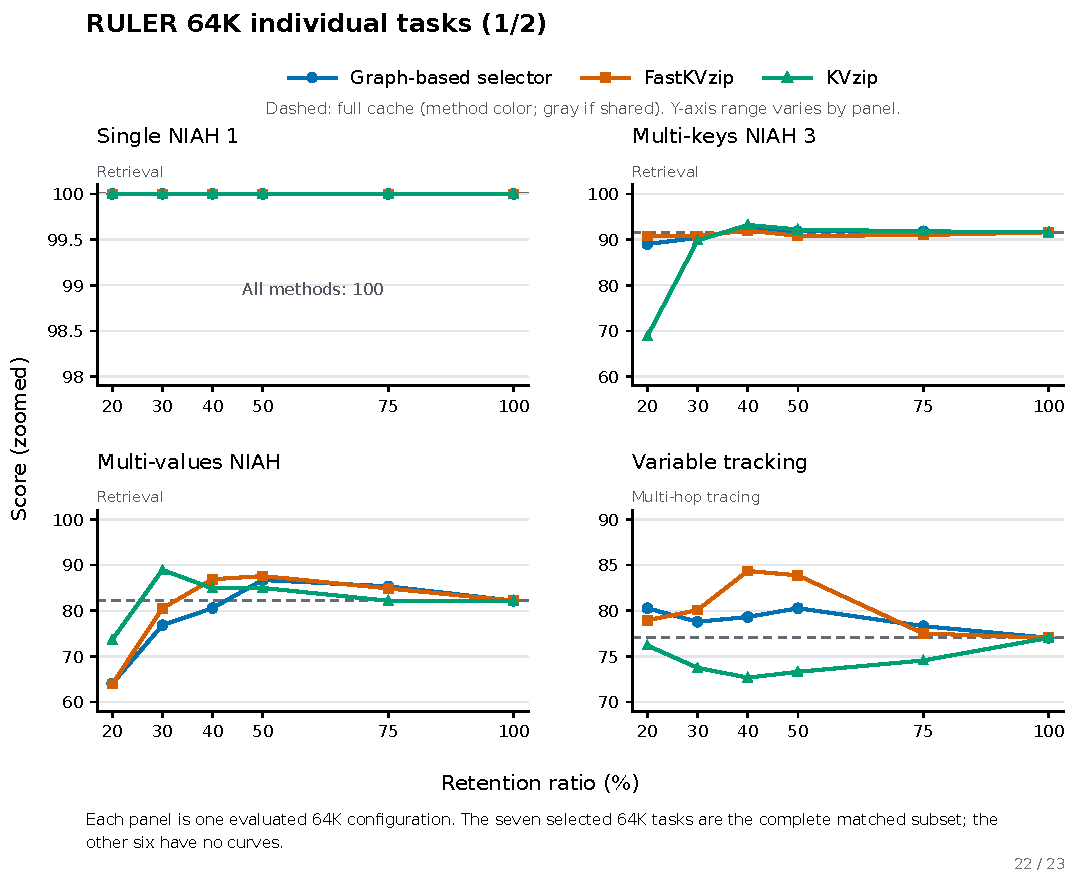
\includegraphics[width=\linewidth]{figures/retention-curves/22-ruler-64k-tasks-1.pdf}
\caption{RULER 64K individual tasks (1/2).}
\label{fig:retention-ruler-64k-tasks-1}
\end{figure}
\clearpage

\begin{figure}[!ht]
\centering
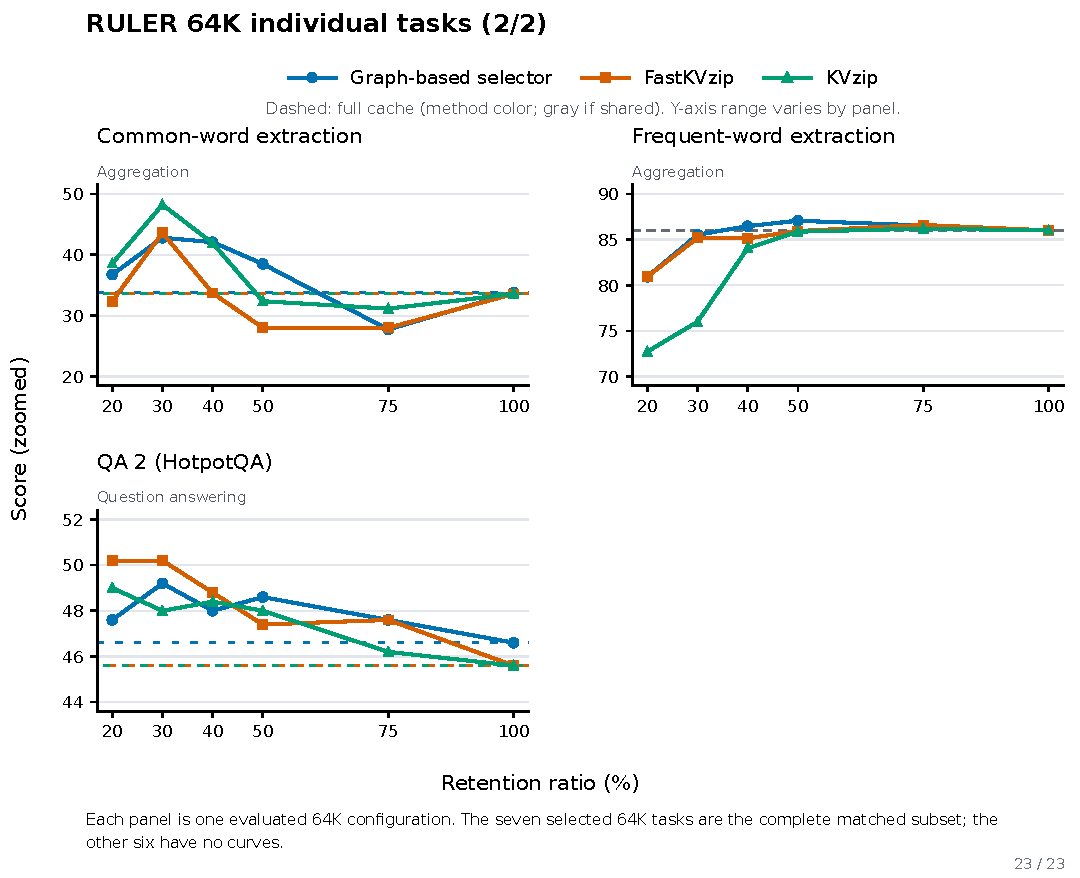
\includegraphics[width=\linewidth]{figures/retention-curves/23-ruler-64k-tasks-2.pdf}
\caption{RULER 64K individual tasks (2/2).}
\label{fig:retention-ruler-64k-tasks-2}
\end{figure}
\clearpage



\end{document}
